%!TEX root = Vorlage_Buch.tex
\chapter{Grills, Smoker und mehr}\label{Chapter1}

	\lettrine[lines=3]{I}{n diesem Kapitel} werde ich auf die Grundlagen des Grillens 
	eingehen. Den Schwerpunkt lege ich dabei auf die
	verschiedenen Grills, Smoker und den Backofen. Alle Geräte ich vorstelle sind 
	in meinem Besitz. So kann ich  meine Erfahrungen und die Eigenheiten meiner
	Geräte weitergeben. Ich werde auf die Handhabung, das Einrichten verschiedener
	Temperaturzonen und die sichere Handhabung der Geräte eingehen.
	
	Ich werde die Besonderheiten der verschiedenen Grills erklären. Die Vorteile 
	und Nachteile herausstellen und euch vermitteln
	weshalb ich mehrere Grills besitze und dazu noch zwei Dutch oven und einen 
	Holzbackofen.
	
	Die Holzkohlen Grills und der Gasgrill können sich gegenseitig ersetzen, 
	außerdem kann Watersmoker durch die Grills
	ersetzt werden. Der Gasgrill eignet sich nicht ganz so gut wie die 
	Holzkohlegrills zum Räuchern, dafür ist es leichter die korrekte Temperatur
	einzustellen.
	
	Die Dutch oven sind mit den Töpfen in der Küche zu vergleichen. D. H. was ich 
	in der Küche auf dem Herd koche kann ich auch im Dutch oven zubereiten. 
	Eine Gulaschsuppe im Dutch oven am Dreibein über offenem Feuer hängend
	hat allerdings ihren eigenen Charme.
	
	Obwohl in diesem Kapitel eine Fülle von Informationen vermittelt werden, erhebe ich keinen Anspruch auf Vollständig- und Allgemeingültigkeit. Es gilt zu Bedenken, dass 
	ich lediglich ein kleines Spektrum der Outdoor-Küche betrachte und die Betrachtungen zu einem Großteil subjektiver Natur sind.



In der folgenden Liste sind die Geräte aufgelistet, die ich euch vorstellen werde.

\begin{itemize}[noitemsep]
	\item Weber Kugelgrill mit einem Durchmesser von 57 cm
	\item Weber Smokey Mountain Water Smoker mit 57 cm Durchmesser
 	\item Napoleon Rogue 425 mit 3 Brennern, mit Seitenkochfeld und 
 	Heckbrenner
	\item Kamado Grill Monolith Classic Pro 2.0
	\item jeweils eine Rotisserie für den Napoleon Gas- und den Weber Kugelgrill
	\item Beefbox Oberflächengrill mit 800°C
	\item Brotbackofen Grundfläche 1 m x 1 m
	\item zwei Dutch oven einen für 4 Personen und einen für bis zu 12 Personen
\end{itemize}

%Wir werden mit dem Holzkohlegrill anfangen. Der Holzkohlegrill tritt in 
%verschiedenen Ausführungen, %Qualitäts-, Ausstattungsvarianten und 
%Preisklassen auf. Diese alle zu behandeln würde den Rahmen 
%sprengen und keinen Mehrwert bringen.

\section{Der Holzkohlegrill}

	Der Holzkohlegrill tritt in verschiedenen Ausführungen, Qualitäts-, 
	Ausstattungsvarianten und Preisklassen auf. 
	Diese alle zu behandeln würde den Rahmen sprengen und keinen Mehrwert 
	bringen.
	
	Ich setze die Holzkohle-Grills Weber Kugelgrill One Touch mit 57 cm 
	Durchmesser und einen Monolith Classic 2.0
	Pro Kamado Grill ein. Daher werden diese Grills in diesem Buch besprochen.
	Diese Geräte unterscheiden sich nur in Details von den Geräten der 
	Mitbewerber, die sich im gleichen Preissegment
	bewegen.  Die Unterschiede liegen meistens im Zubehör und in der 
	Ausstattung.
	
	Wir fangen mit dem Kugelgrill (siehe Abbildung~\vref{fig:Kugelgrill}) an. Der Aufbau des Kugelgrills ist recht simpel. 
	Es handelt sich um eine zweigeteilte
	Kugel, einem Kessel und dem Deckel. Kessel wie Deckel sind mit 
	Lüftungsschlitzen ausgestattet die je 
	nach gewünschter Temperatur eingestellt werden können und die im  Kessel 
	für die Be- und im Deckel für 
	Entlüftung sorgen. Im Kessel sind zwei Roste zu finden, der untere, kleinere 
	Rost ist der Kohlerost, der 
	obere ist für das Grillgut. Da je nach Grillgut verschiedene Heizzonen 
	eingerichtet werden sollten, muss der
	Kugelgrill groß genug sein. Mein Kugelgrill hat einen Innendurchmesser von 
	57cm, was ich persönlich für 
	eine optimale Größe halte, wenn mehr als zwei Leute am Tisch sitzen. Für zwei 
	Leute geht auch der kleinere 
	Kugelgrill mit 37cm Durchmesser.

\subsection{Die unterschiedlichen Heizzonen} \label{Heizzonen}
	
	Je nach Grillgut wird mit verschiedenen Heizzonen gearbeitet. Ein 
	kurzgebratenes Steak benötigt eine 
	andere Temperatur als ein langsam gegartes Hähnchen. Soll etwas fertig 
	gegart werden legt man es 
	besser auf die indirekte Hitze damit das Grillgut nicht verbrennt. Halten wir 
	fest, es gibt also starke, 
	mittlere und niedrige Hitze. Die direkt oder indirekt genutzt werden kann. In der 
	unten stehenden Tabelle 
	sind die Temperaturbereiche für die Hitzestufen angegeben. Ich benutze zwei 
	Methoden um die 
	gewünschte Hitze zu ermitteln. Erstens mit dem Thermometer, was eine sehr 
	genaue Bestimmung ist. 
	Zweitens mit der Hand. Stellt euch eine Cola-Dose, die auf dem Rost steht, vor. 
	In dieser Höhe haltet Ihr 
	die Hand über den Grill, in der dritten Spalte der Tabelle sind die Zeiten 
	festgehalten, nachdem die Hand 
	weggezogen wird,  weil die Hitze sonst zu stark ist. Diese Methode ist 
	erstaunlich präzise und liefert 
	recht sichere Ergebnisse.  Es sollte allerdings keine Mutprobe oder ein 
	Wettbewerb daraus gemacht werden.
	Niemand sollte sich bei dieser Methode verletzen.
\newline
 
\begin{table*}[htpb]
\centering
\caption{Handtest}
\label{tab:Handtest}
\begin{tabular}{lcr}
		\multicolumn{3}{c}{\textbf{Temperaturbereiche}}		\\
\hline										\\
\emph{Hitze}		&\emph{Temperaturbereich}		& \emph{Die Handprobe}	\\
Stark				& 230 - 290 °C					& 2 - 4 Sekunden	\\
Mittel              & 175 - 230 °C					& 5 - 7 Sekunden	\\
Niedrig				& 120 - 175 °C					& 8 - 10 Sekunden	\\
\end{tabular}
\end{table*}
%\newline

	Es gibt einige Methoden den Kugelgrill zu befeuern. Je nach Grillgut kann 
	entschieden werden mit welcher 
	Temperatur direkt oder indirekt gegrillt werden soll. Im folgenden werde ich die 
	Methoden vorstellen und euch
	zeigen für welches Grillgut sie geeignet sind.
	
	Es gibt die Zwei-Zonen-Glut. Dabei schichtet man, wie auf 
	Abbildung~\vref{fig:ZweiZonen} zu sehen ist, auf 
	der einen Seite des Grillrostes die Holzkohle oder die Briketts so auf, dass der 
	gewünschte Temperaturbereich 
	erreicht wird. Die andere Hälfte ist die indirekte Hitze. Somit kann auf der 
	direkten Seite scharf angegrillt und 
	auf der indirekten Seite das Grillgut fertig gegart werden. Die Methode ist für 
	Kurzgebratenes bestens 
	geeignet. So können dicke Steaks nach scharfem angrillen langsam auf die 
	richtige Garstufe gezogen werden.

\begin{figure}[htbp]
	\centering
	\begin{minipage}{.5\textwidth}
		\centering
		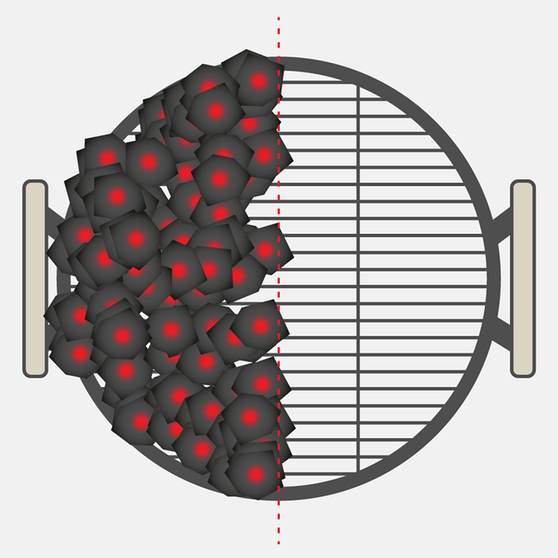
\includegraphics[width=.5\linewidth]{pics/ZweiZonen}
		\captionof{figure}{Zwei-Zonen-Glut}
		\label{fig:ZweiZonen}
	\end{minipage}%
	\begin{minipage}{.5\textwidth}
		\centering
		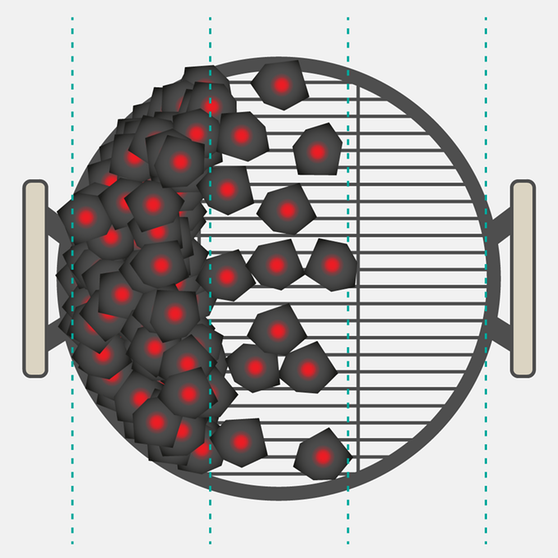
\includegraphics[width=.5\linewidth]{pics/DreiZonen}
		\captionof{figure}{Drei-Zonen-Glut}
		\label{fig:DreiZonen}
	\end{minipage}%
\end{figure}

	Für eine Drei-Zonen-Glut zu werden 2/3 des Kohlerosts mit Holzkohle oder 
	Briketts bedeckt, entsprechend der 
	Abbildung~\vref{fig:DreiZonen}. Die Glut wird am Rand so hoch gestapelt, dass 
	eine starke Hitze entsteht und fällt zur Mitte 
	hin 
	ab. So hat man am Rand eine direkte starke Hitze, in der Mitte eine direkte 
	mittlere Hitze und indirekte Hitze auf der anderen 
	Seite.

\begin{figure}[htbp]
	\centering
	\begin{minipage}{.5\textwidth}
		\centering
		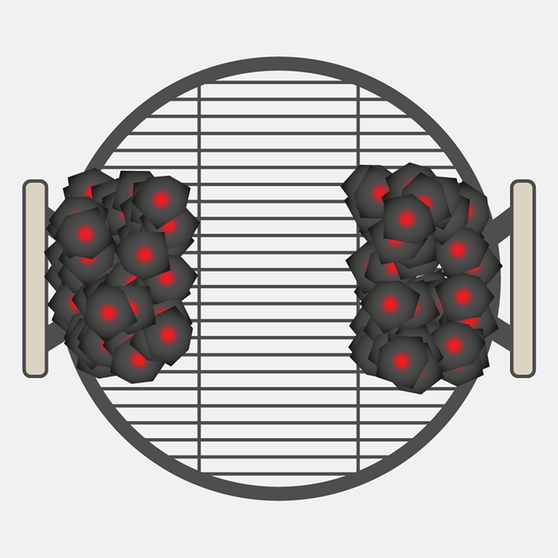
\includegraphics[width=.5\linewidth]{pics/ZweiZonengeteilt}
		\captionof{figure}{Geteilte Zwei-Zonen-Glut}
		\label{fig:ZweiZonengeteilt}
	\end{minipage}%
	\begin{minipage}{.5\textwidth}
		\centering
		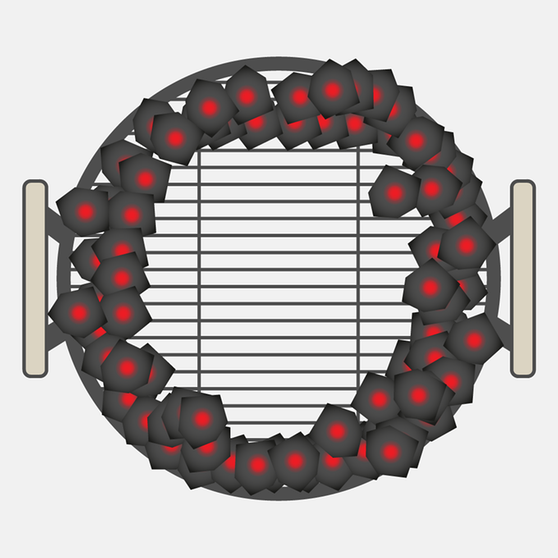
\includegraphics[width=.5\linewidth]{pics/FeuerRing}
		\captionof{figure}{Der Feuer-Ring}
		\label{fig:FeuerRing}
	\end{minipage}%
\end{figure}

	Die Methode der geteilten Zwei-Zonen-Glut, siehe 
	Abbildung~\vref{fig:ZweiZonengeteilt}, hat gleich zwei Vorzüge. Zum 
	einen verteilt sich
	die indirekte Hitze gleichmäßig zum anderen kann in der Mitte des Grills eine 
	feuerfeste Tropfschale platziert werden. Die mit 
	Wasser, Bier, 
	Fruchtsaft etc. befüllt werden kann, das aromatisiert das Grillgut, schützt es 
	vor dem Austrocknen und hält die Temperatur 
	konstant.
	
	Während die geteilte Zone für größere Braten und die Rotesserie ideal ist, ist 
	die Variante Feuer- Ring wie in 
	Abbildung~\vref{fig:FeuerRing}
	dargestellt, besonders geeignet für das berühmte Brathähnchen, das man auf 
	eine halbvolle Bierdose oder auf einen 
	Hähnchenhalter stülpt
	und im geschlossenen Grill indirekt grillt.

\begin{figure}[htbp]
	\centering
	\begin{minipage}{.5\textwidth}
		\centering
		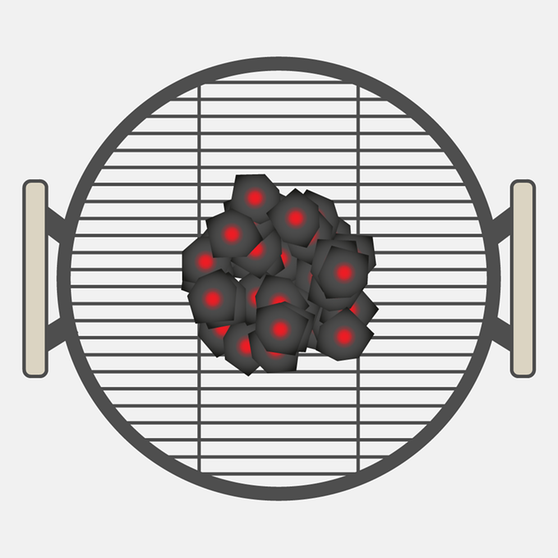
\includegraphics[width=.5\linewidth]{pics/BullsEye}
		\captionof{figure}{Das Bulls Eye}
		\label{fig:BullsEye}
	\end{minipage}%
	\begin{minipage}{.5\textwidth}
		\centering
		\includegraphics[width=.5\linewidth]{pics/MenionRIng}
		\captionof{figure}{Der Menion-Ring}
		\label{fig:MenionRing}
	\end{minipage}%
\end{figure}

	Das Bulls Eye ist das Gegenteil des Feuer-Rings, siehe 
	Abbildung~\vref{fig:BullsEye} und ist bestens geeignet für 
	Kurzgebratenes. Der Grill
	sollte dafür aber groß genug sein um eine indirekte Zone entsprechender 
	Größe zu bekommen.
	
	Der ">heilige Gral"< des indirekten Grillens ist der Menion-Ring, siehe 
	Abbildung~\vref{fig:MenionRing}. Richtig angewendet, 
	kann man damit
	im geschlossenen Grill bis zu 20 (!) Stunden indirekt bei knapp 120°C grillen, 
	ohne Briketts nachlegen zu müssen. Briketts 
	zweireihig anordnen. 
	Die Briketts müssen sich unbedingt berühren. Die Starterbriketts (weiß im Bild) 
	bereitet man im Anzündkamin vor (zur Hälfte 
	füllen), sie werden
	an den Rand des Rings platziert. So glüht der komplette Ring Stück für Stück 
	durch. Ideal z. B. für ">The holy trinity of BBQ"< 
	\ bestehend aus 
	Beef Brisket, Pulled Pork und Spareribs.

\subsection{Handhabung des Holzkohlegrills}

	Ein Holzkohlegrill kann mit Holzkohle oder Briketts (ich werde im weiteren 
	Verlauf nur von Holzkohle reden, Briketts sind im 
	gleichen Maße 
	betroffen) beheizt werden. 
	Der Unterschied liegt an der Hitze und der Brenndauer. Die Holzkohle brennt in 
	der Regel heißer, die Briketts dagegen länger. 
	Die Entscheidung welches Medium genutzt wird ist keine reine 
	Geschmackssache, sondern auch zum Teil des Grillgutes 
	gewidmet. Dazu später 
	mehr.

	\paragraph{Methoden des Anfeuern}

	Es gibt verschiedene Arten den Grill anzufeuern, zum Einen gibt es die 
	Möglichkeit die Holzkohle respektive die Briketts auf 
	dem Grillrost,
	entsprechend der gewünschten Heizzonen wie in Abschnitt~\vref{Heizzonen} 
	erklärt, anzurichten. Dann die Holzkohle mit 
	einem flüssigen oder 
	festen Grillanzünder
	an zu zünden. Diese gibt es sowohl mit Paraffin und/ oder Petroleum oder 
	schadstoffe frei. Hat man welche aus Paraffin oder 
	solche die Petroleum 
	beinhalten, muss auf eine 
	vollständige Verbrennung der Grillanzünder geachtet werden.
	
	Dann gibt es die Möglichkeit die angerichtete Holzkohle mit einem Heißluftföhn 
	zu erhitzen. Dabei ist man allerdings auf eine 
	Stromquelle 
	angewiesen, was sich m.E. als Nachteil
	erweisen kann.
	
	Als weitere Möglichkeit gibt es die elektrischen Grillanzünder, die an einen 
	Tauchsieder erinnern. Diese werden zwischen die 
	Kohlen gelegt und an 
	eine Steckdose angeschlossen. 
	Innerhalb weniger Minuten ist die Holzkohle durchgeglüht. Auch dabei ist eine 
	Stromquelle nötig.
	
	Meine präferierte Methode ist der Anzündkamin.  Darin wird die Holzkohle 
	aufgeschichtet und mit einem Grillanzünder 
	angezündet. Ich benutze 
	Anzünder aus gewachster Holzwolle. 
	Oder ein ölgetränktes Blatt von der Küchenrolle, mit dem ich den Grillrost leicht 
	eingefettet habe. Die Holzkohle glüht von unten nach oben 
	durch, mit Hilfe der 
	Luft die wie in einem Kamin von unten nach oben steigt
	und den wichtigen Sauerstoff transportiert. Ist die Holzkohle durchgeglüht, 
	man erkennt es an der grauen Asche auf den 
	Kohlestücken, wird die 
	Kohle in den Grill geschüttet und 
	entsprechend der gewünschten Heizzone arrangiert.

	\paragraph{Reinigen nach dem Grillen}

	Nach dem Grillen ist in der Regel noch genug Hitze im Grill um den Rost 
	nochmal auf Temperatur zubringen, dass die Reste 
	des Grillguts 
	weitestgehend verbrennen. 
	Mit einer Messingdrahtbürste kann dann der Rost abgebürstet werden.
	
	Sobald der Grill abgekühlt und die Glut vollständig erloschen ist, sollte die 
	Asche entfernt werden. Da die Asche 
	hygroskopisch ist und Wasser 
	selbst aus 
	der Luft anzieht. Durch die Feuchte die sich in der Asche bildet kommt es nach 
	einiger Zeit zur Rostbildung. Das wird durch 
	entfernen der Asche 
	vermieden.
	Weitere Reinigung ist nicht notwendig, es sei den der Grill ist sehr stark 
	verschmutzt und es haben sich schon relativ dicke 
	Anbackungen 
	entwickelt.
	Die Anbackungen können mit einer Holzspachtel, die beim Raclette verwendet 
	wird, abgeschabt werden.
	
	
		\begin{figure}[htbp]
		\centering
		\begin{minipage}{1\textwidth}
			\centering
			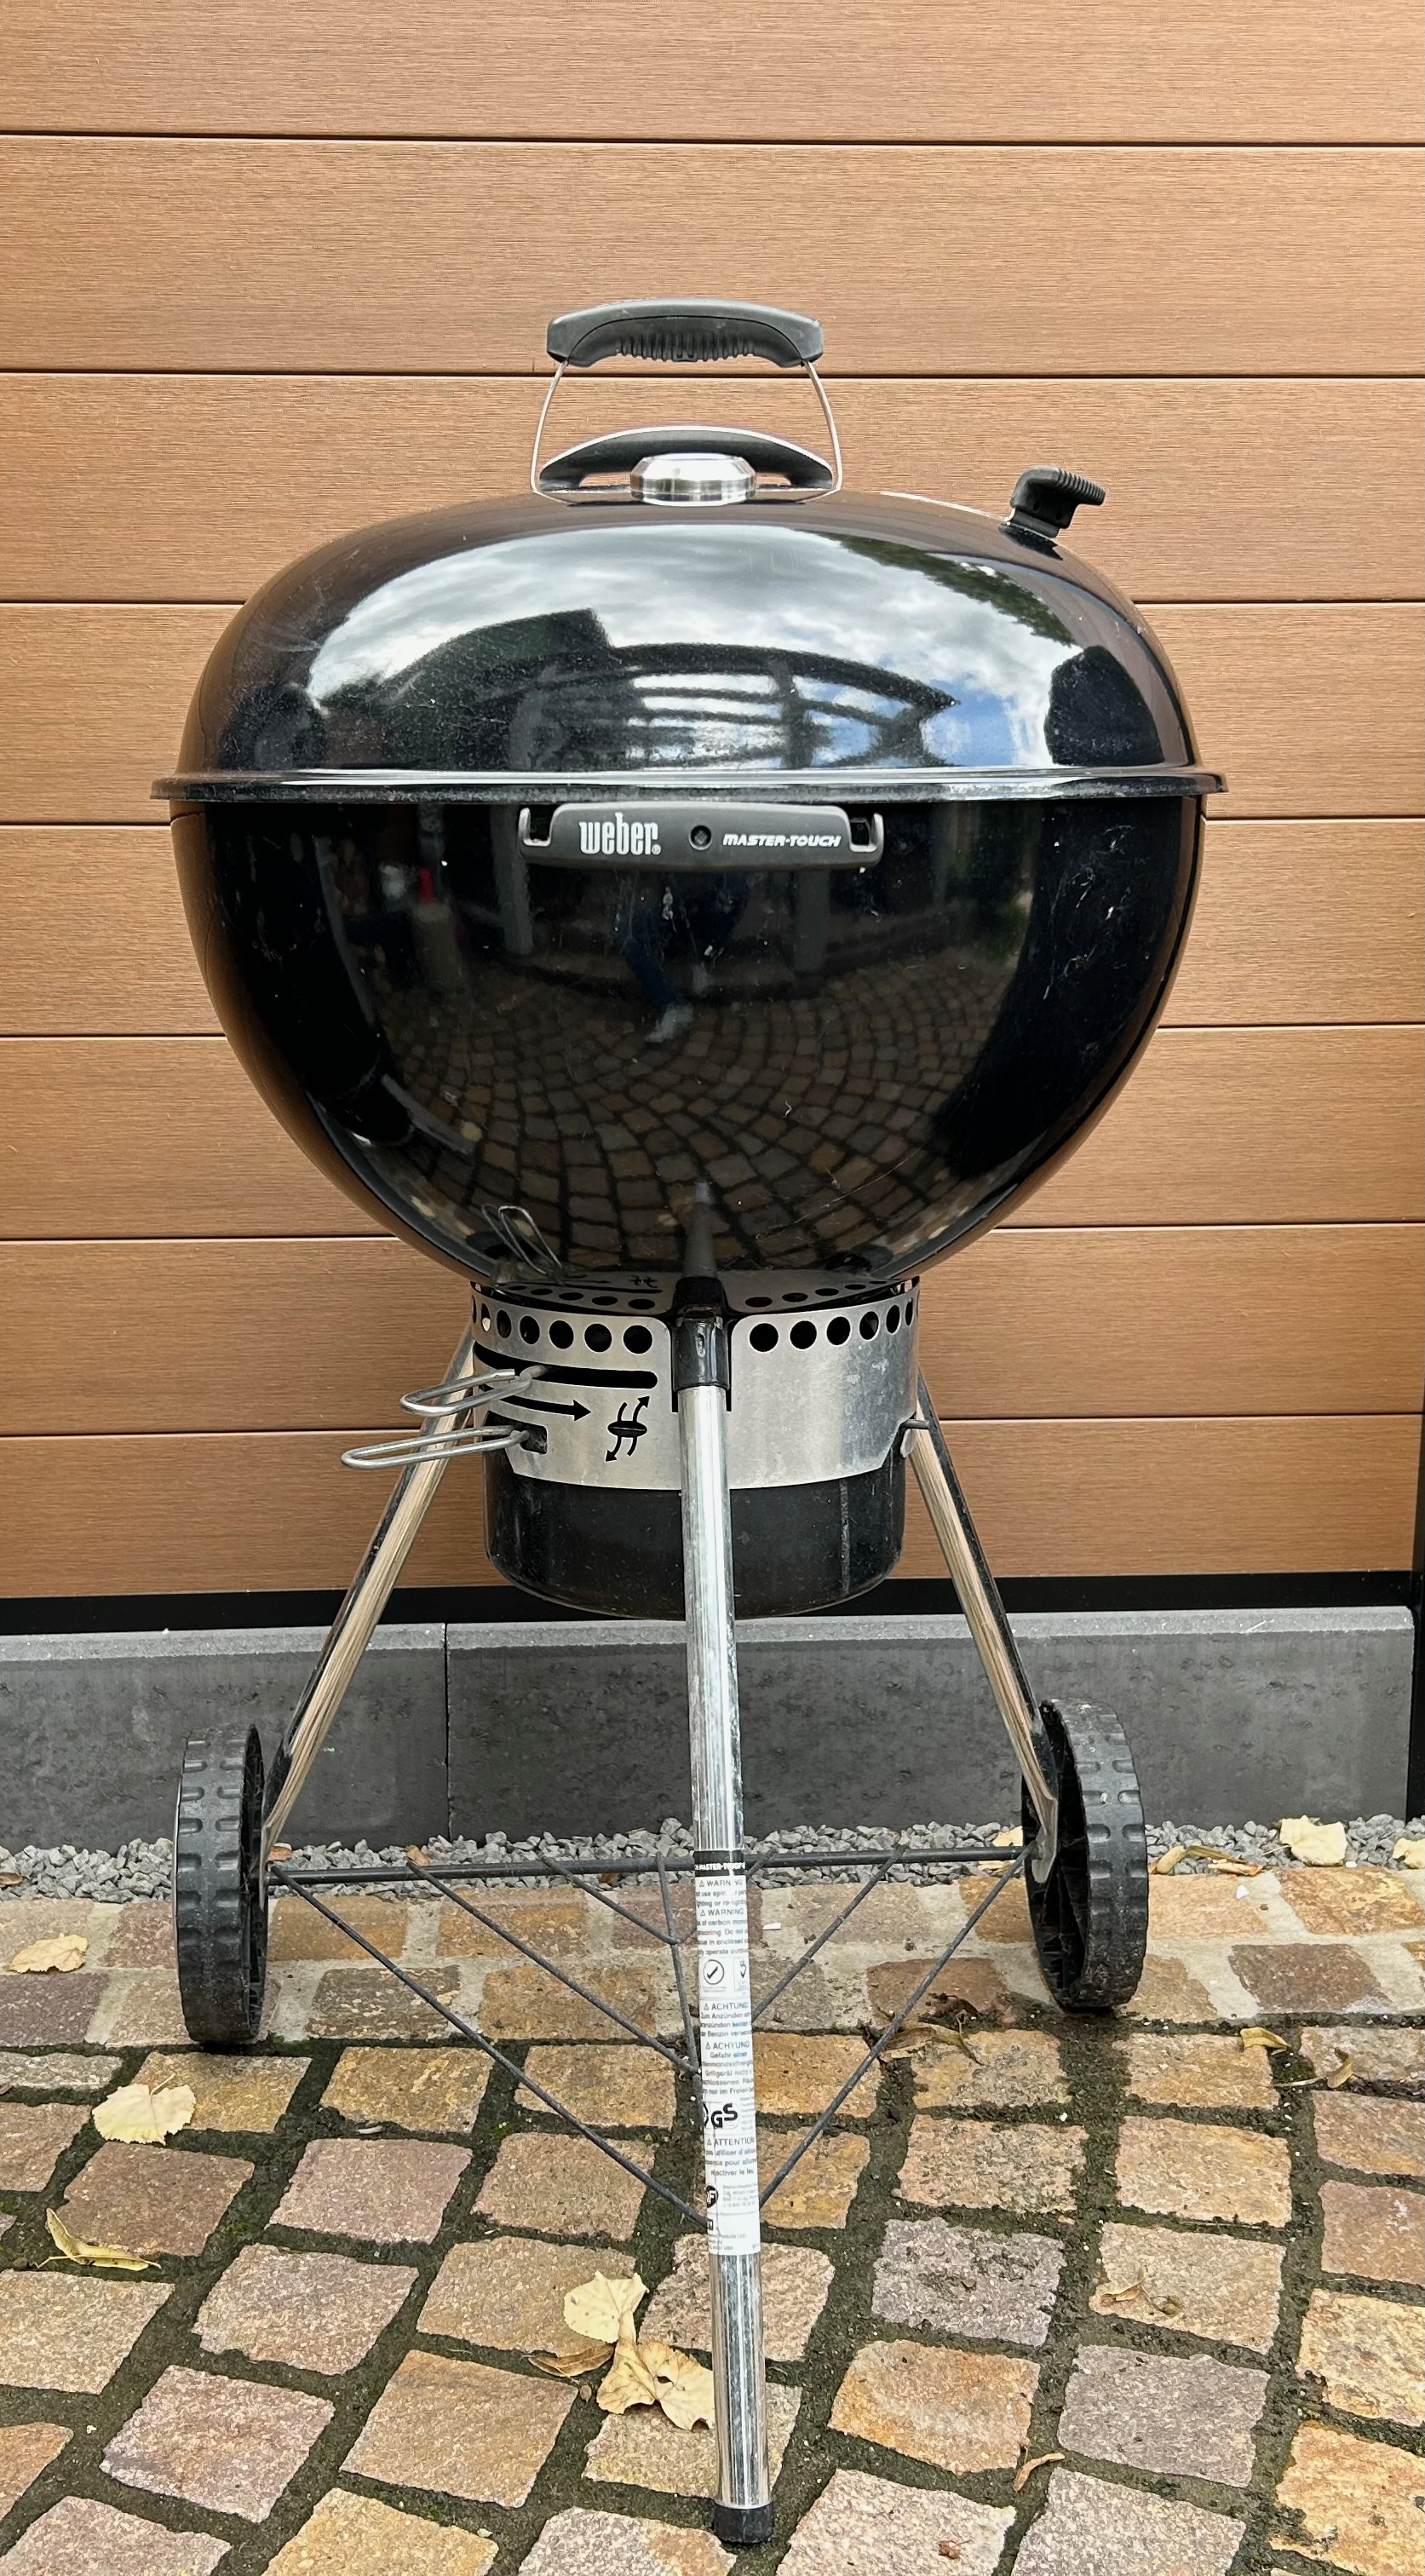
\includegraphics[width=.6\linewidth]{pics/Kugelgrill}
			\captionof{figure}{Kugelgrill Weber One Touch}
			\label{fig:Kugelgrill}
		\end{minipage}%
	\end{figure}
	
	\newpage

\section{Der Kamado Grill}

	Das Prinzip des Keramik-Grills ist bereits mehrere tausend Jahre alt. Es begann 
	mit einem Loch, das 
	mit Steinen, später mit Lehm und Ton ausgekleidet und als weitere Entwicklung 
	mit 
	einem Rand versehen wurde um das Feuer vor Wind zu schützen. 
	Im Laufe von einigen tausend Jahren wurde in der Edo-Zeit in Japan (Anfang 
	des 17ten Jahrhunderts 
	bis Mitte des 19ten Jahrhunderts) aus dem Feuerloch der Mushi-Kamado, die 
	heutige Form
	der Kamado-Grills.
	
	Im Nachkriegsjapan wurde von einem in Japan stationierten Amerikaner, dieser 
	Reis-Dampfgarer mit 
	einem Rost zum Grill umgebaut. Mit den Amerikanern kam dieser ">Grill"< nach 
	Amerika und begann 
	einen Siegeszug um die Welt. Über den Teich kam der Grill erst um das 
	Millennium herum, als 
	Kochgerät für die Spitzengastronomie (vorrangig in Belgien und der 
	Niederlande). Der Keramik-Grill (siehe Abbildung ~\vref{fig:Keramikgrill}) ist heute
	auch für grillbegeisterte Privatleute erschwinglich und in der Regel nur ein paar 
	Mausklicks und 
	mehrere Hundert bis wenige tausend Euro entfernt.
	
	Der Keramik-Grill ist eiförmig und wird mit einen Gestell, das Nest genannt 
	wird, geliefert. Falls der 
	Einbau in eine Außenküche gewünscht ist, kann er auch ohne Gestell geliefert 
	werden.
	Da die Grills aus Keramik bestehen werden sie im fernen Osten, genau 
	genommen China, das über 
	eine mehre tausend Jahre alte Tradition der Keramikverarbeitung verfügt, 
	gefertigt. Es gibt 
	verschiedene Hersteller von Keramik-Grills, die Big-Player in diesem Segment 
	sind Big Green Egg, 
	Kamodo Joe und Monolith . Die beiden erstgenannten sind amerikanische 
	Unternehmen, ohne in 
	überschwänglichen Patriotismus zu verfallen ist meines Erachtens der Monolith 
	im Augenblick der am 
	Besten durchdachte Keramik-Grill im Kreis der Big-Player. Der niederländische 
	Hersteller IQ liefert 
	mehr Zubehör mit, kann allerdings nicht mit den drei genannten Marken mit 
	halten. Entgegen der 
	landläufigen und von den Herstellern propagierten Meinung die Keramik spiele 
	eine große Rolle, ist 
	dem nicht so. Punkten können die verschiedenen Hersteller nur mit dem 
	Zubehör, der mehr oder 
	weniger gut durchdacht ist, oder eben Funktionen die die Mitbewerber nicht 
	oder nicht in der Qualität 
	anbieten. So verfügt der Monolith über das beste Rostsystem, das beste 
	System zur Einbringung von 
	Räucher-Chips und Asche-Entnahme-System. Des Weiteren ist ein eingebauter 
	Adapter für den BBQ-
	Guru angebracht. Als Kritikpunkt kann gesagt werden, dass das Nest kein 
	Design-Highlight darstellt.
 
\subsection{Handhabung des Kamado-Grills}

	Die Handhabung des Kamado-Grills unterscheidet sich in wenigen Punkten 
	zum Kugelgrill. Im Kamado-
	Grill werden die indirekten Zonen in der Regel über zwei halbkreisförmige 
	Deflektorsteine realisiert. 
	Das heißt es werden keine Heizzonen durch die Lage der Holzkohle 
	eingerichtet. Bei dem Monolith Pro Serie ist
	es möglich den Grillkorb zu unterteilen und den Korb nur halb mit Kohle 
	zufüllen. Durch die Teilbaren 
	Roste und Deflektorsteine können auch auf diese Weise direkte und indirekte 
	Zonen eingerichtet 
	werden.
	Der nächste Unterschied ist, dass der Deckel im Betrieb nur einen Spalt weit 
	geöffnet werden darf bis 
	ein Luftaustausch stattgefunden hat und der Grill komplett geöffnet werden 
	kann. Bei zu schnellem Öffnen kann es durch den einströmenden 
	Sauerstoff zu einem Flammenschlag kommen. Daher besteht ein gewisses 
	Verletzungsrisiko.

\subsection{Anfeuern des Kamado-Grills}

	Es wird empfohlen eine Holzkohle, die frei von chemischen Zusatzstoffen ist zu 
	verwenden. Die Holzkohle
	sollte eine homogene Größe der Kohlestücke haben und außerdem großstückig 
	sein. Briketts sind für Keramikgrill
	nicht zu empfehlen, da sie Bindemittel enthalten, die sich in der Keramik 
	festsetzen. Außerdem ist die
	Hitze der Briketts zu gering für den Keramik-Grill.
	
	Hier eine Auflistung der Bindemittel die in Briketts eingesetzt werden.

	\begin{itemize}[noitemsep]
		\item Stärke
		\item Ton
		\item Melasse
		\item Holzteer
		\item Pech
	\end{itemize}
 
  
	Bei einem Longjob wie z.B. Beef Brisket, Pulled Pork oder Spare Ribs wird der 
	Feuerkorb befüllt. Der 
	Feuerkorb kann mehr Kohle aufnehmen als der  Kohlekorb. Bei kürzeren 
	Garzeiten, aber höheren 
	Temperaturen sollte der Kohlekorb eingesetzt werden. Da weniger Kohle 
	benötigt wird. Bedingt durch 
	den Kohlekorb wird die Holzkohle optimal mit Sauerstoff versorgt.
	Angefeuert werden kann der Grill mit Bio-Anzündern. Wenn schnell eine hohe 
	Hitze, siehe 
	Abbildung~\vref{fig:Große}, erreicht werden soll, werden 3 Anzünder benötigt. 
	Die in einem Dreieck auf 
	die Kohle gelegt und angezündet werden. Die Be- und Entlüftung wird komplett 
	geöffnet.
	
	Bei geringer Hitze wird nur ein Grill-Anzünder benötigt. Auch hier werden die 
	Lüftungsschlitze ganz 
	geöffnet. Bevor der Grill die Wunschtemperatur erreicht, sollte der Grill durch 
	schließen der 
	Lüftungsschlitze (bitte nicht ganz, da sonst das Feuer erstickt) abgefangen 
	werden. Das Abkühlen eines 
	Kamado-Grills dauert, durch die hohe Wärmekapazität der Keramik, sehr lange.
	
	Alternativ zu den Grillanzündern kann auch ein Looftlighter zum Entzünden der 
	Holzkohle verwendet 
	werden. Ich benutze einen Heißluftföhn, der für das Anzünden von Grillkohle 
	geeignet ist.

\begin{figure}[htbp]
	\centering
	\begin{minipage}{.5\textwidth}
		\centering
		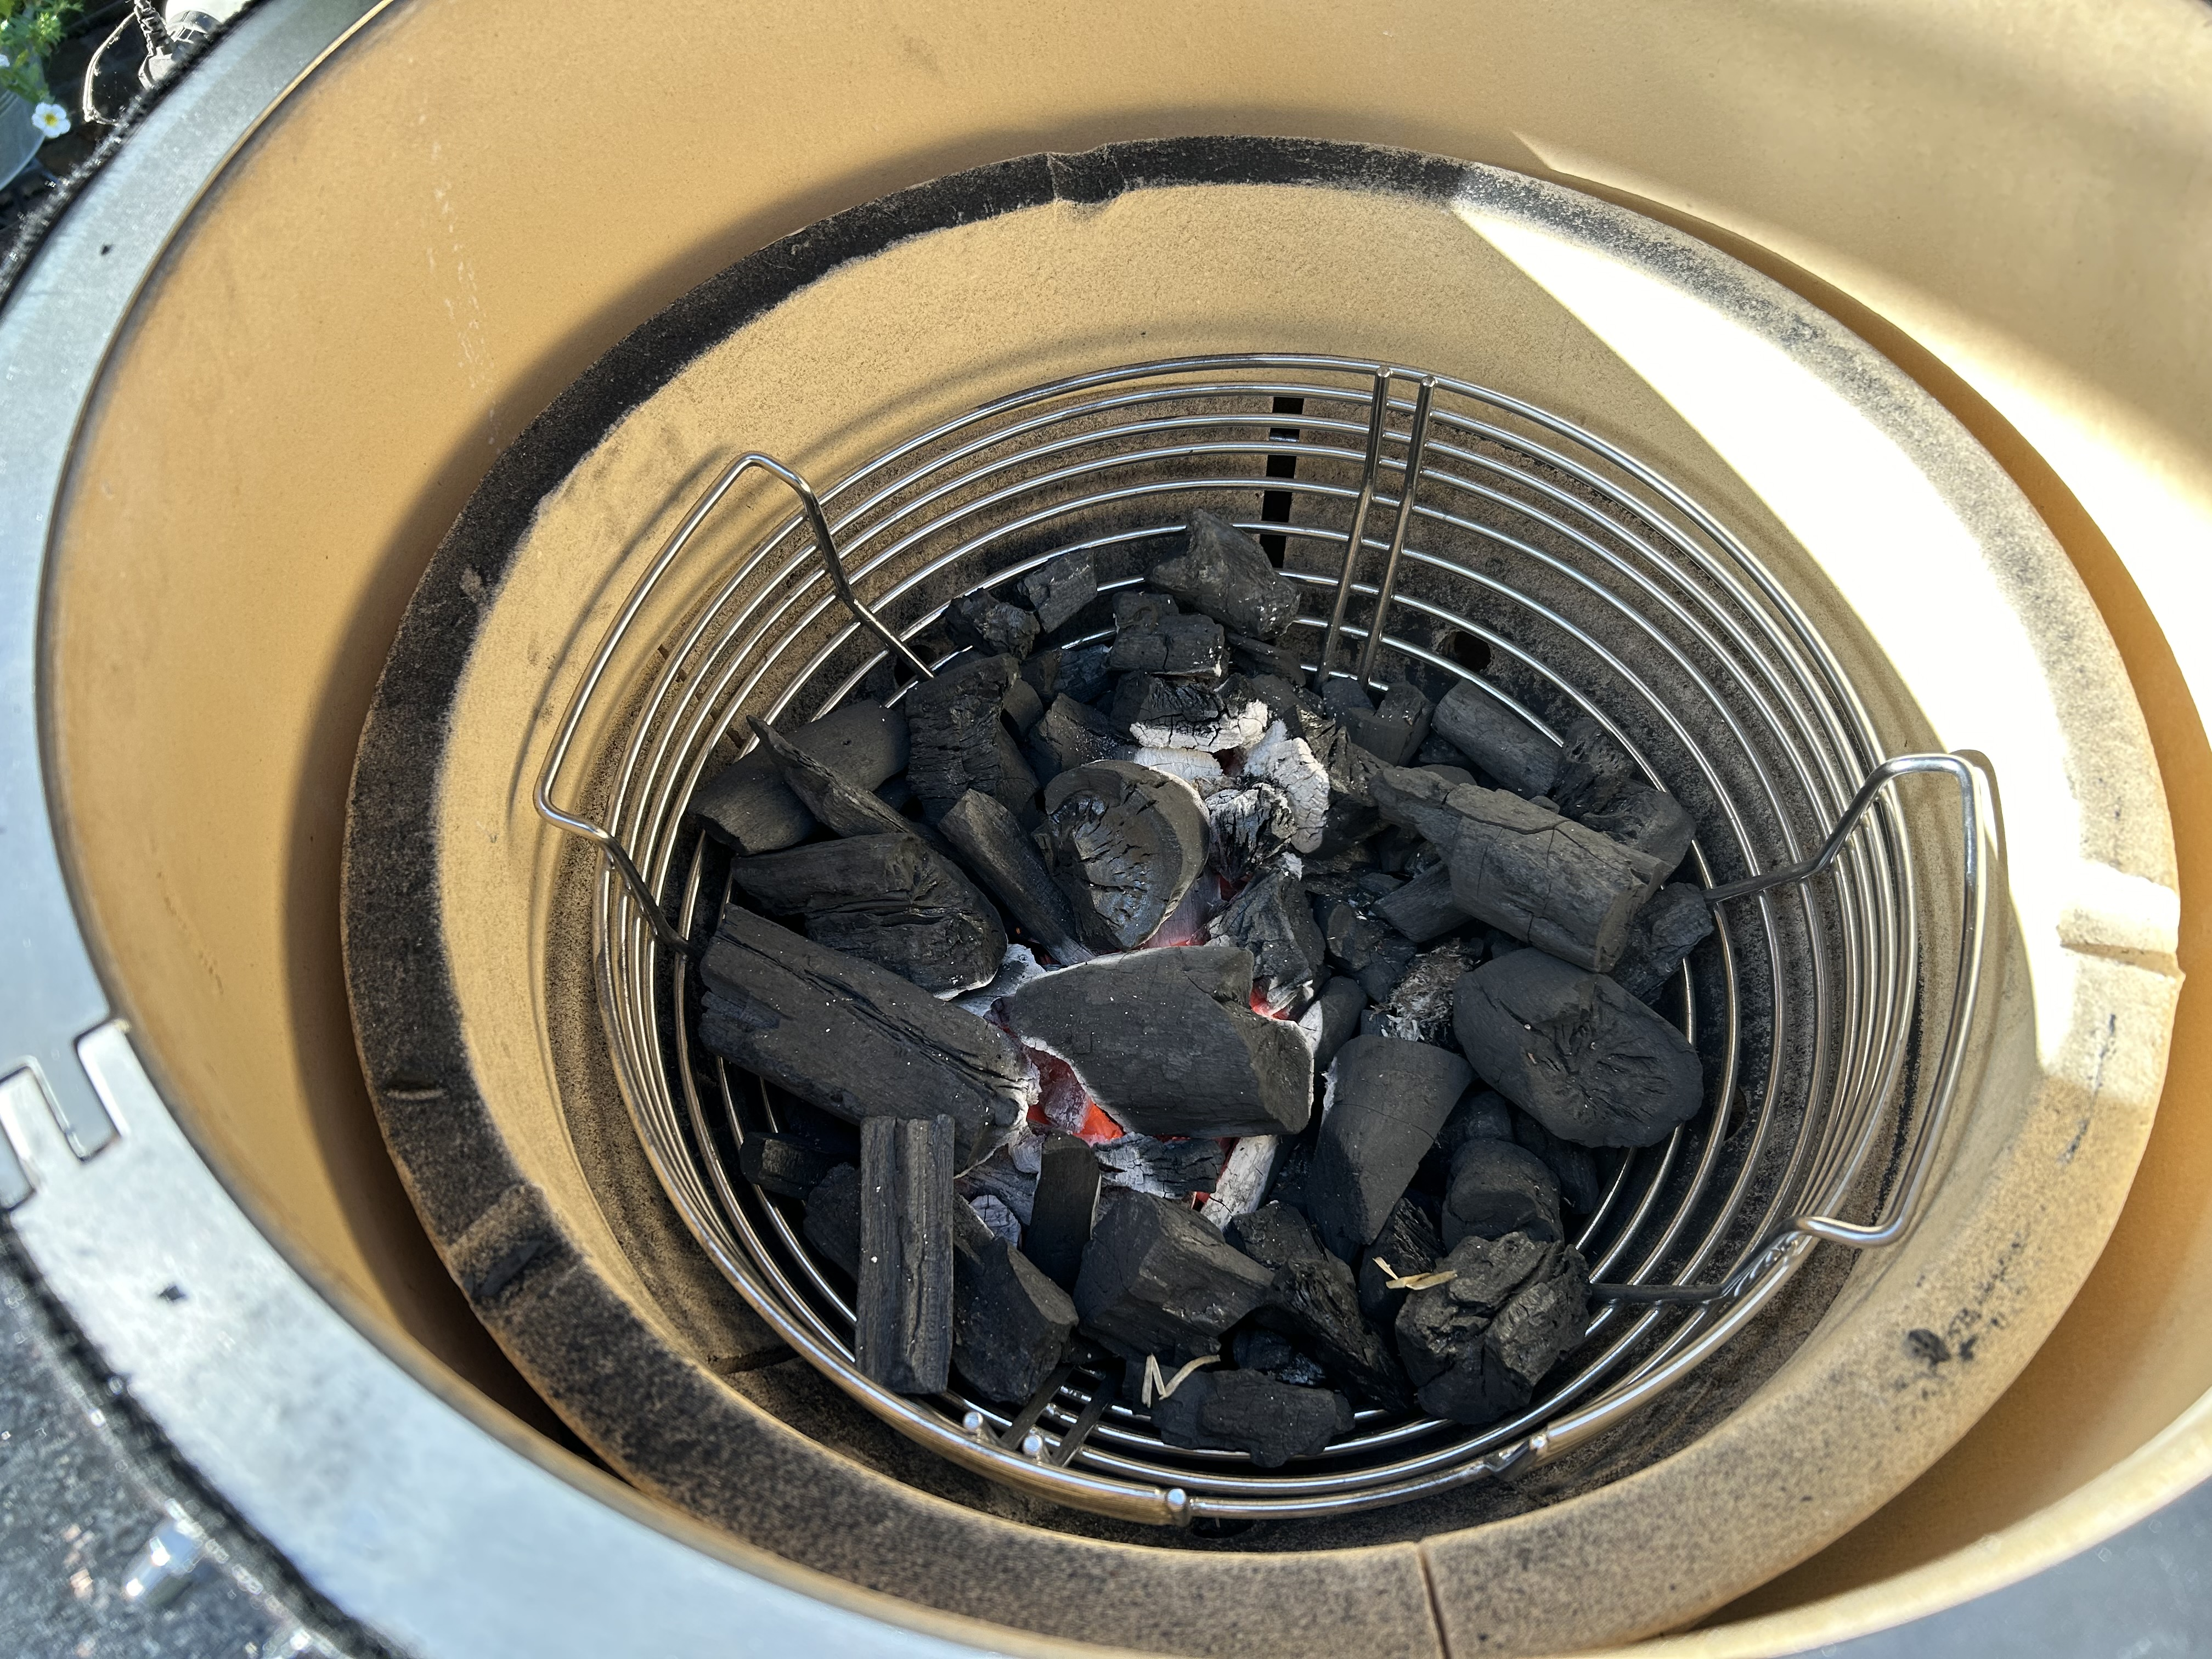
\includegraphics[width=.5\linewidth]{pics/Anfeuern_Monolith}
		\captionof{figure}{Anfeuern Monolith}
		\label{fig:Anfeuern}
	\end{minipage}%
	\begin{minipage}{.5\textwidth}
		\centering
		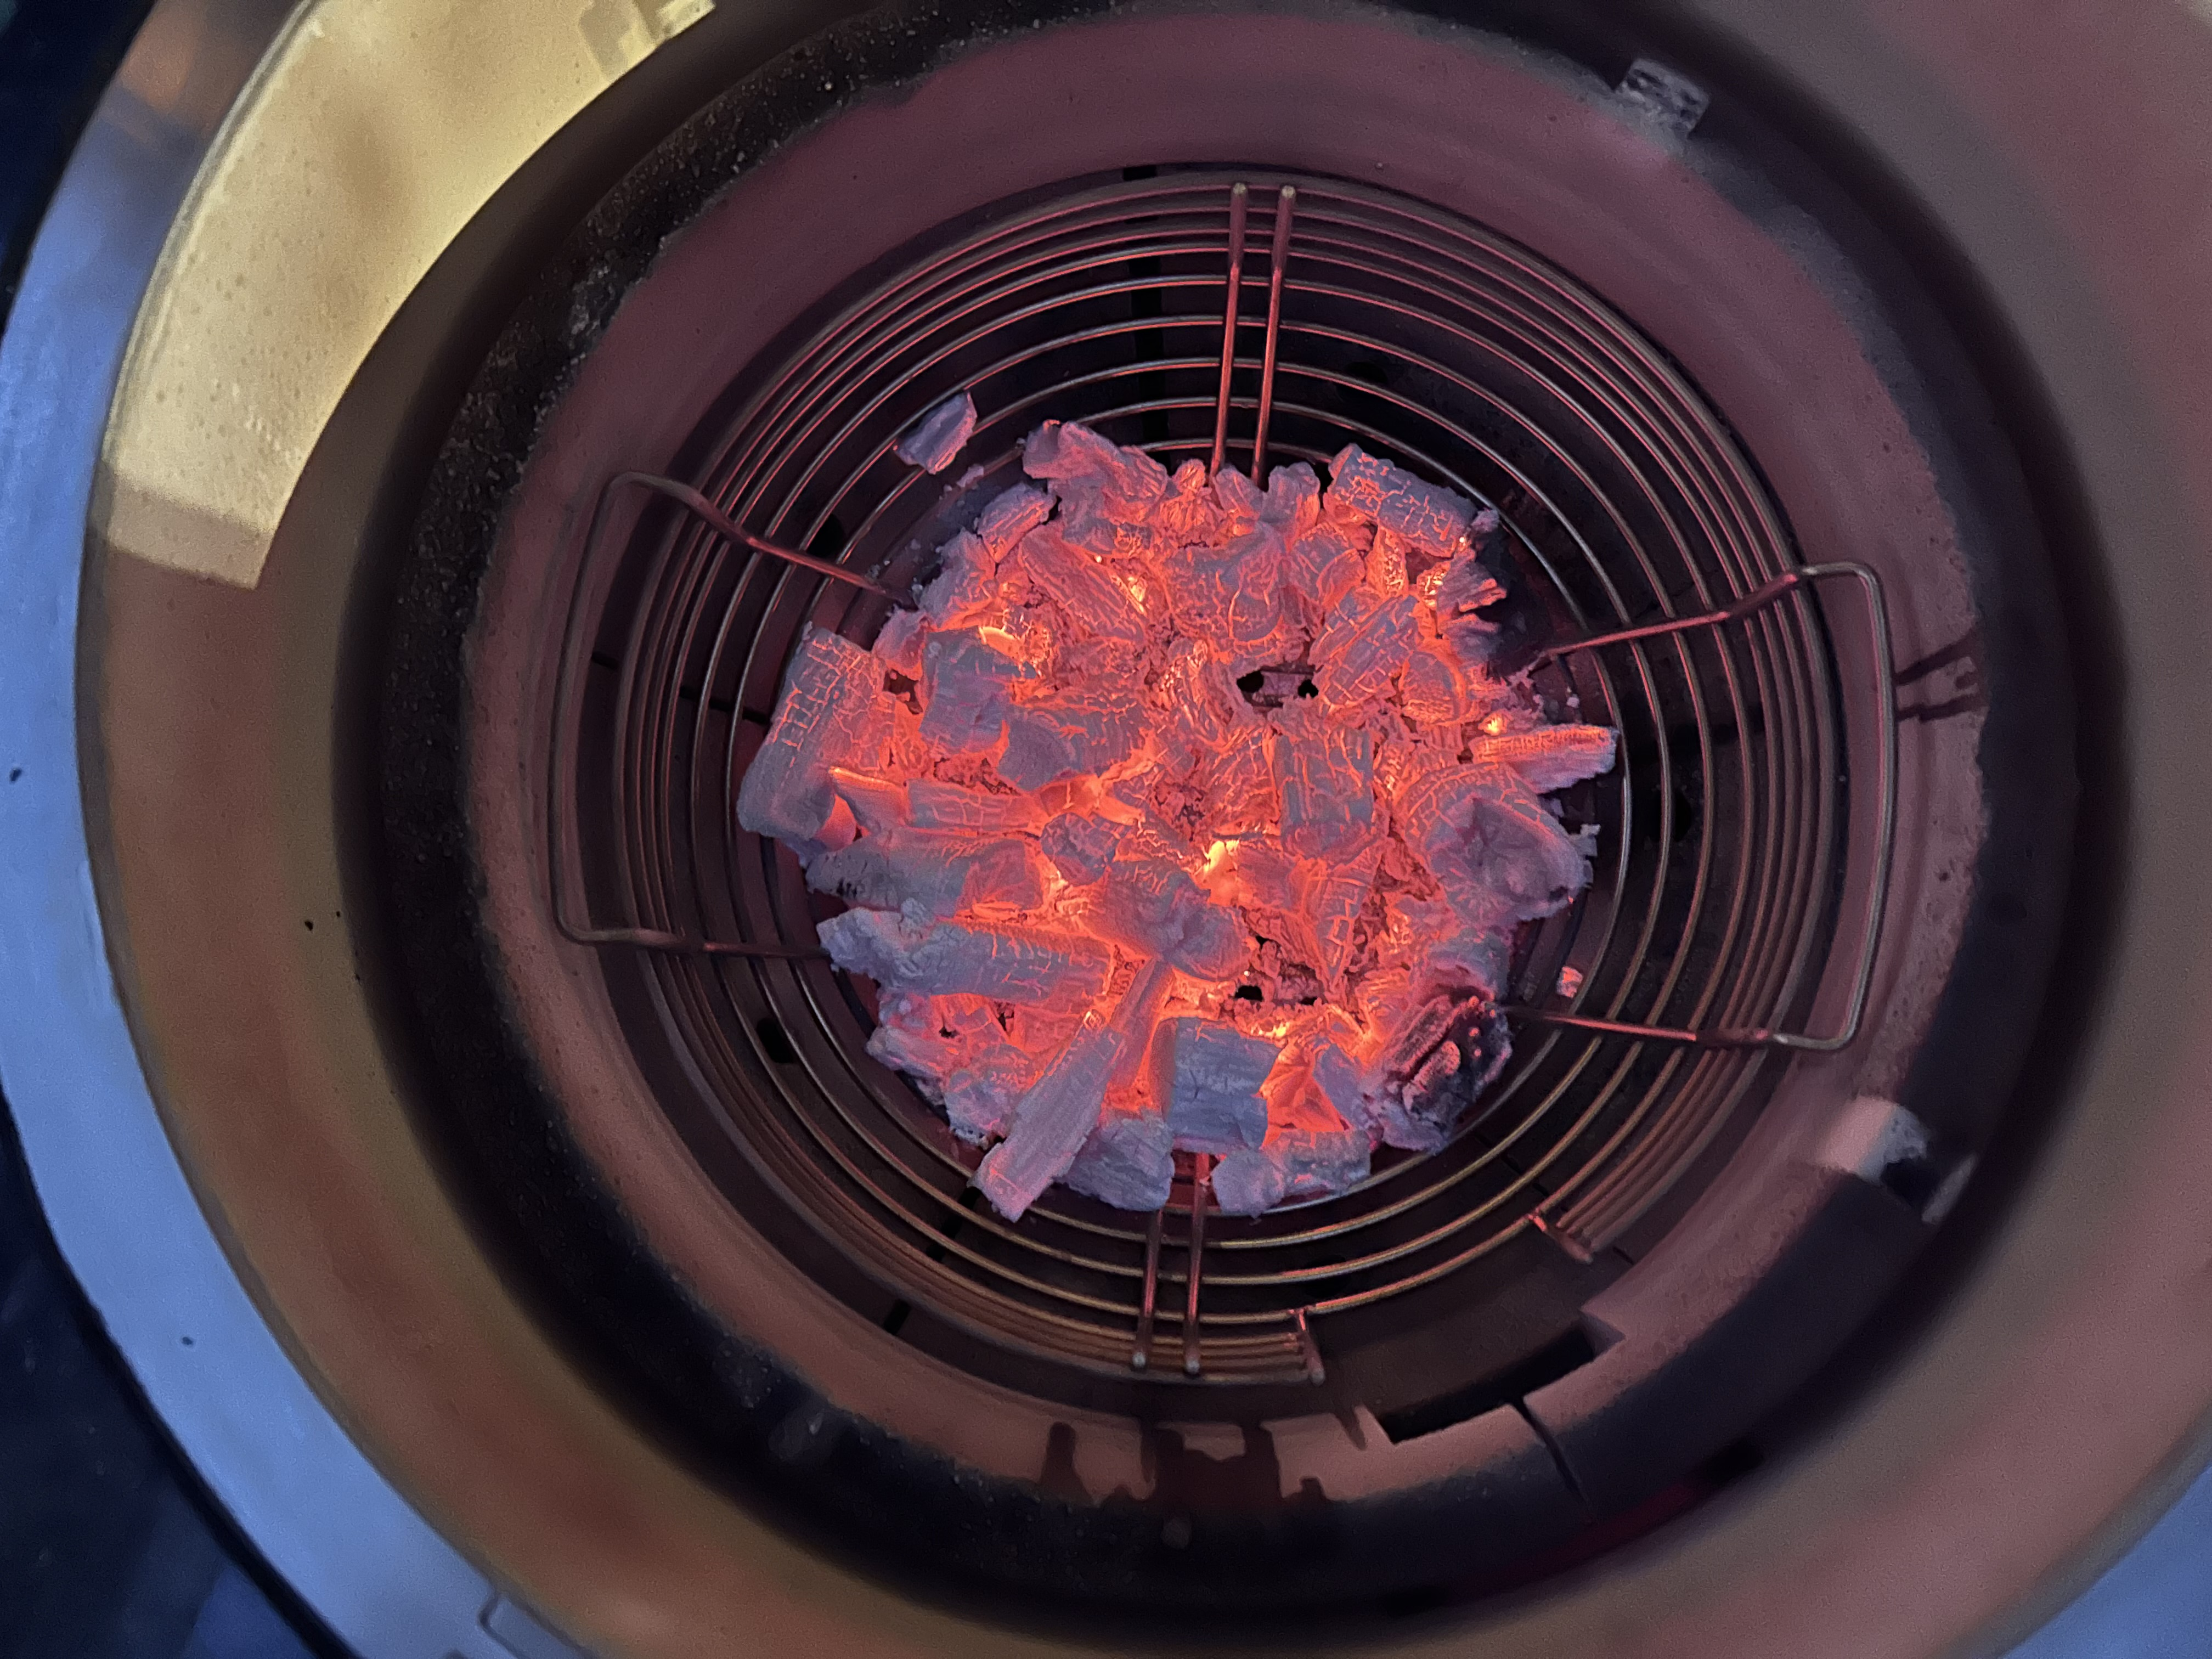
\includegraphics[width=.5\linewidth]{pics/Große_Hitze}
		\captionof{figure}{Große Hitze}
		\label{fig:Große}
	\end{minipage}%
\end{figure}
\newpage

\subsection{Reinigen des Kamado-Grills}

	Das Reinigen erfolgt durch Aufheizen und Abbürsten der Roste und spülen der 
	Abtropfwannen. Die 
	Reinigung der Keramik erfolgt durch starkes Erhitzen (Pyrolyse bei ca. 400°C).
	
	\begin{figure}[htbp]
		\centering
		\begin{minipage}{1\textwidth}
			\centering
			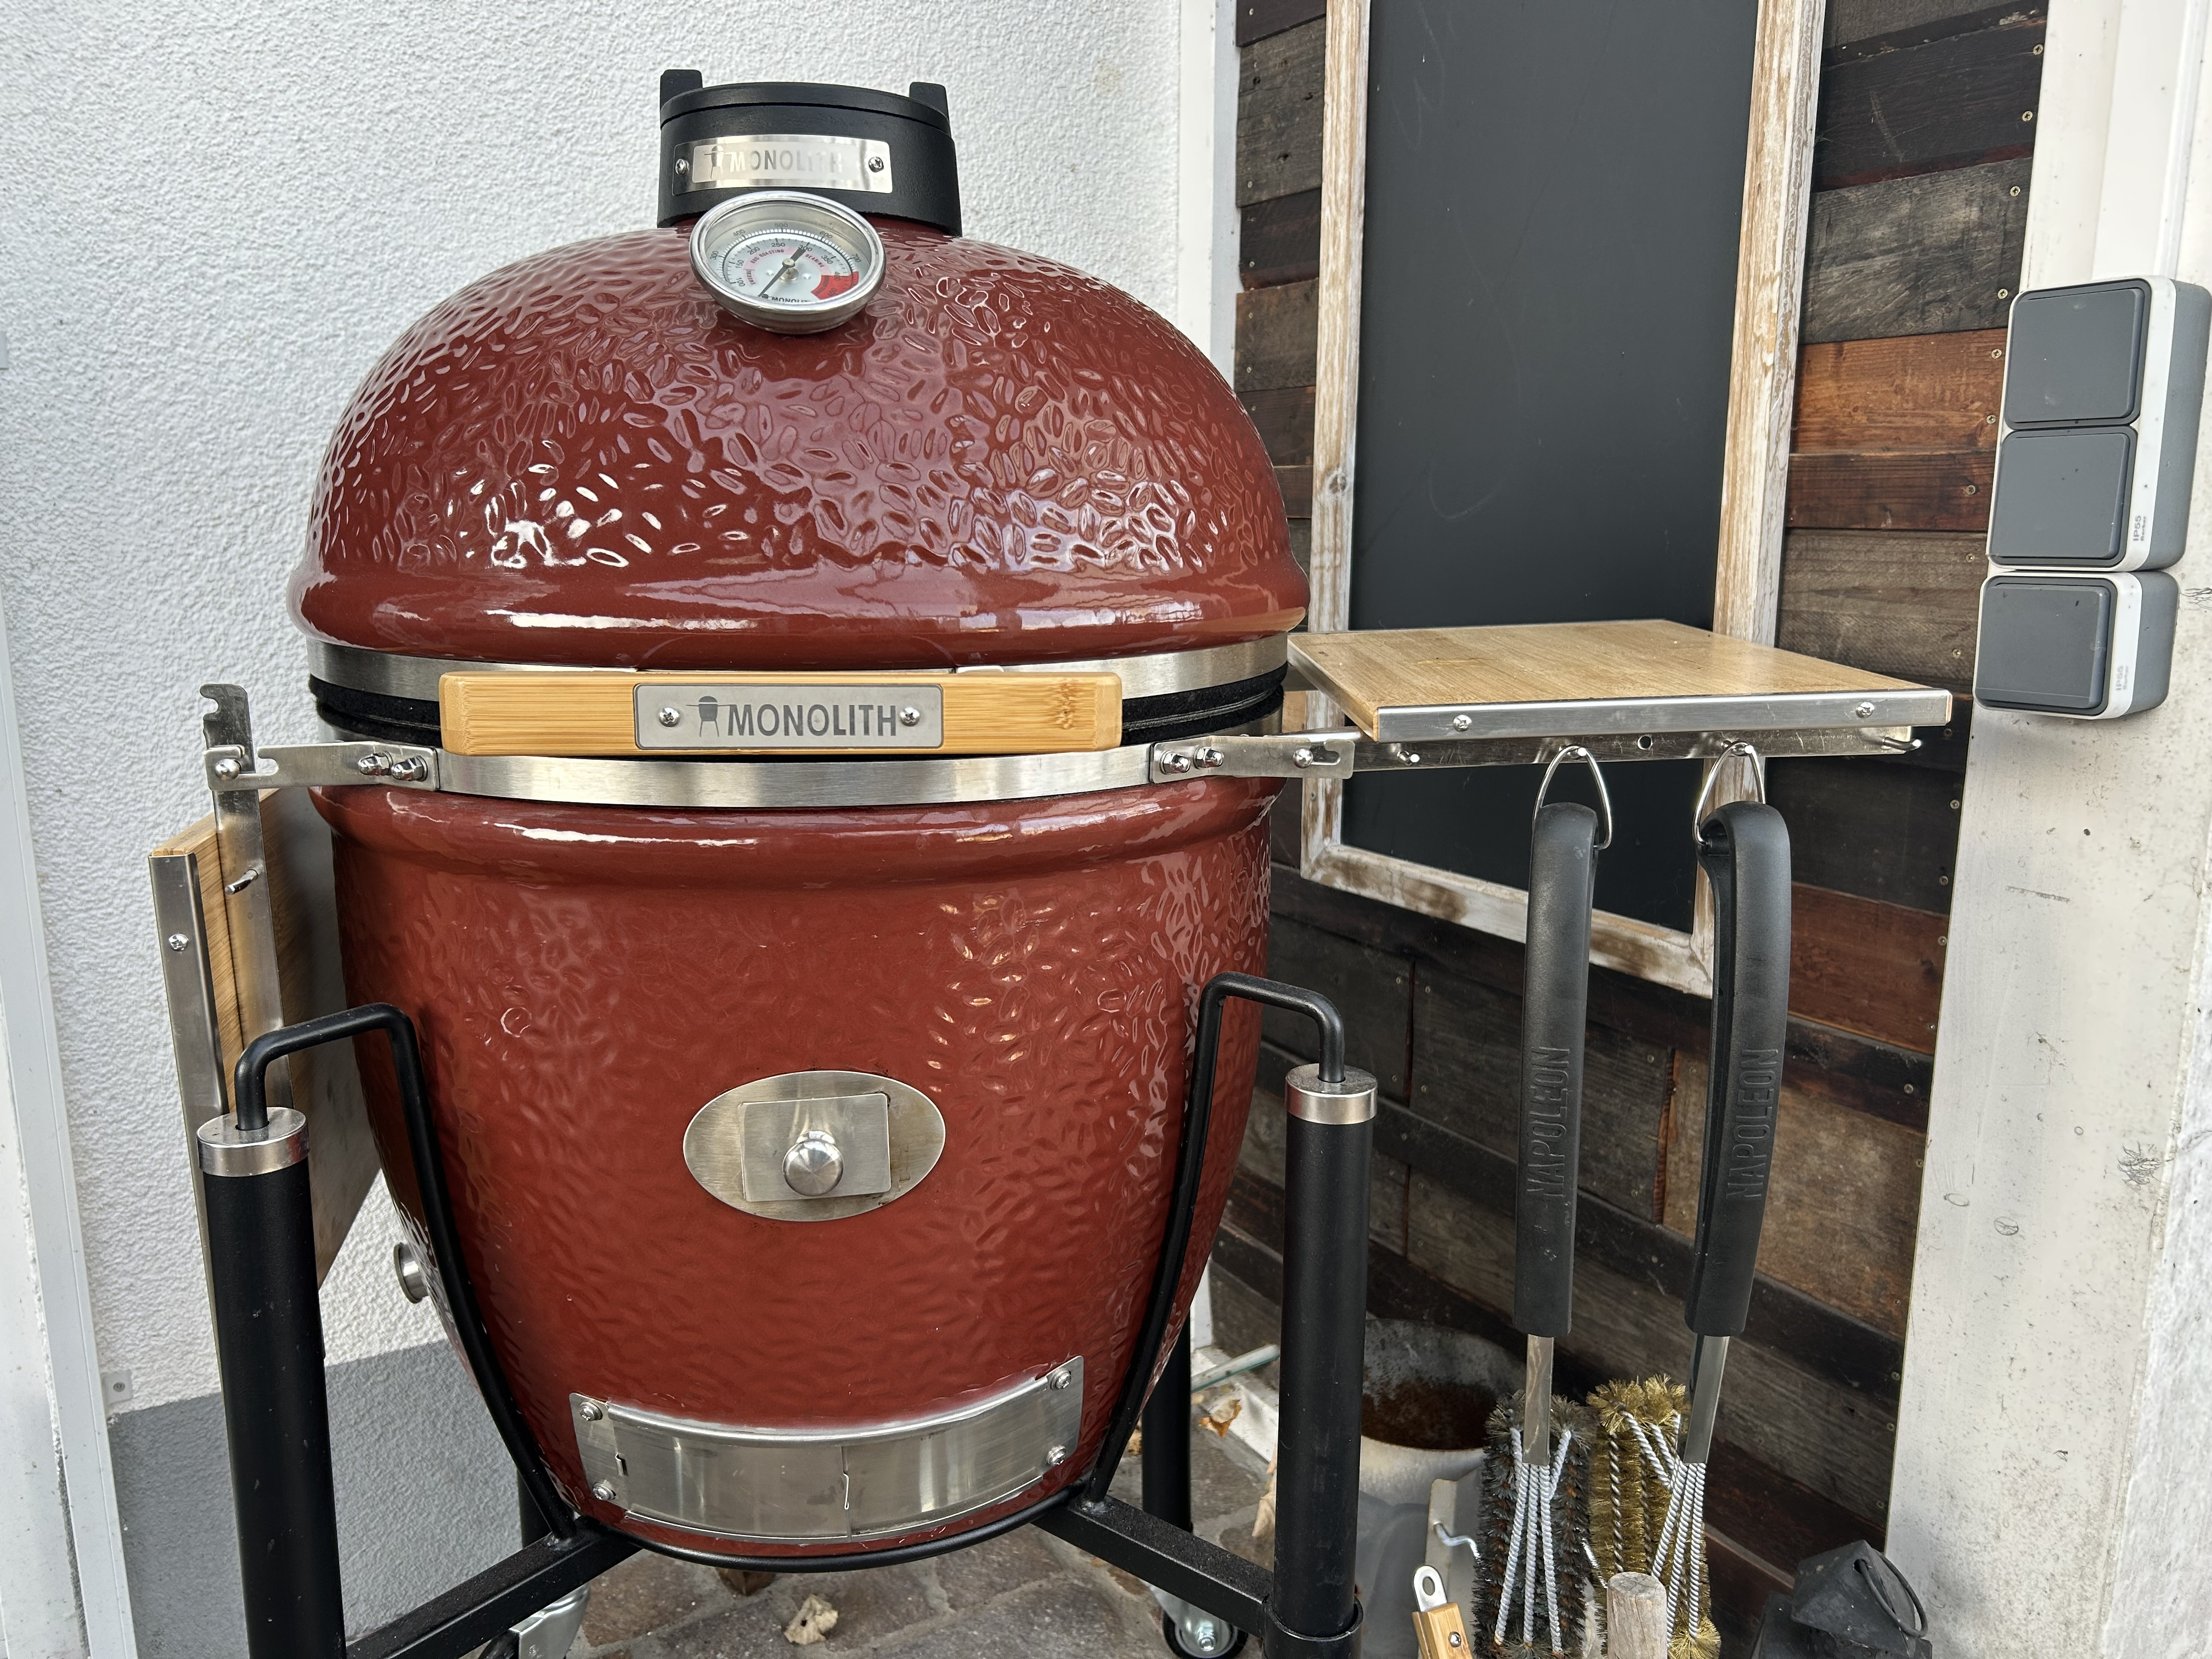
\includegraphics[width=1\linewidth]{pics/Keramikgrill}
			\captionof{figure}{Kamado-Grill Monolith Classic 2 Pro}
			\label{fig:Keramikgrill}
		\end{minipage}%
	\end{figure}
\newpage
\section{Der Gasgrill}

	Die Modellvielfalt und die Ausstattungsvarianten der Gasgrills ist gefühlt noch 
	umfangreicher als bei den 
	Holzkohle-Grills. Es gibt Gasgrills die für 
	deutlich unter 100 €\ zu haben sind. Und den Oberklassengrills, die 
	hochmodern, aus bestens 
	verarbeiteten und qualitativ hochwertigen Materialien
	hergestellt sind und preislich jenseits der 15.000~€\ liegen. Dazwischen gibt es 
	Gasgrills in allen 
	erdenklichen Ausstattungsvariationen, Qualitätsstufen und Preisklassen. 
	

\subsection{Was benötige ich bei einem Gasgrill unbedingt?} 

	Hier ist die 
	Antwort gar nicht so leicht. 
	Es kommt auf die Ansprüche an. Habe ich 
	vor mich mit dem Grillen intensiver zu beschäftigen komme ich um indirektes 
	Grillen nicht herum. In diesem Fall sind 
	mindestens drei Hauptbrenner 
	Pflicht.  Bei zwei Brennern ist der Abstand von der indirekten Grillfläche zu der 
	direkten Grillfläche zu klein. Besser ist ein Grill 
	mit vier 
	Hauptbrennern. Ich persönlich besitze einen Grill mit drei Hauptbrennern, 
	einem Seitenkochfeld siehe Abbildung~\vref{fig:Napoleon}und einem Heckbrenner. Da 
	ich einen 
	Oberflächengrill mit einer Maximaltempera~tur von 800°C besitze, konnte ich 
	mir den Keramikbrenner in meinem Gasgrill 
	sparen. 
	
	Sollte der Gasgrill nicht ausreichen, zum Beispiel für ein Beef Brisket Full 
	Packer, nehme ich den Kugelgrill oder den Smoker 
	zur Hand. Aus diesem 
	Grund musste der Gasgrill nicht sehr groß dimensioniert sein. 
	
	Eine Schlauchbruchsicherung, die gegen ausströmendes Gas schützt, ist 
	meines Erachtens für die Sicherheit unerlässlich 
	und sollte unbedingt nachgerüstet 
	werden. 
	Auch bei hochwertigen Grills im gehobenen Preissegment sind 
	Schlauchbruchsicherungen siehe 
	Abbildung~\vref{fig:Sicherung} so gut wie nicht im 
	Lieferumfang enthalten. Dieses Bauteil ist für kleines Geld, ca. 13,00 € bis 
	20,00~€, erhältlich. Die Sicherheit des Grillers 
	oder umstehenden 
	Personen sollte diese geringe Investition wert sein. Im 
	professionellen Bereich ist so ein Bauteil gesetzlich gefordert.

\begin{figure}[htbp]
	\centering
	\begin{minipage}{.5\textwidth}
		\centering
		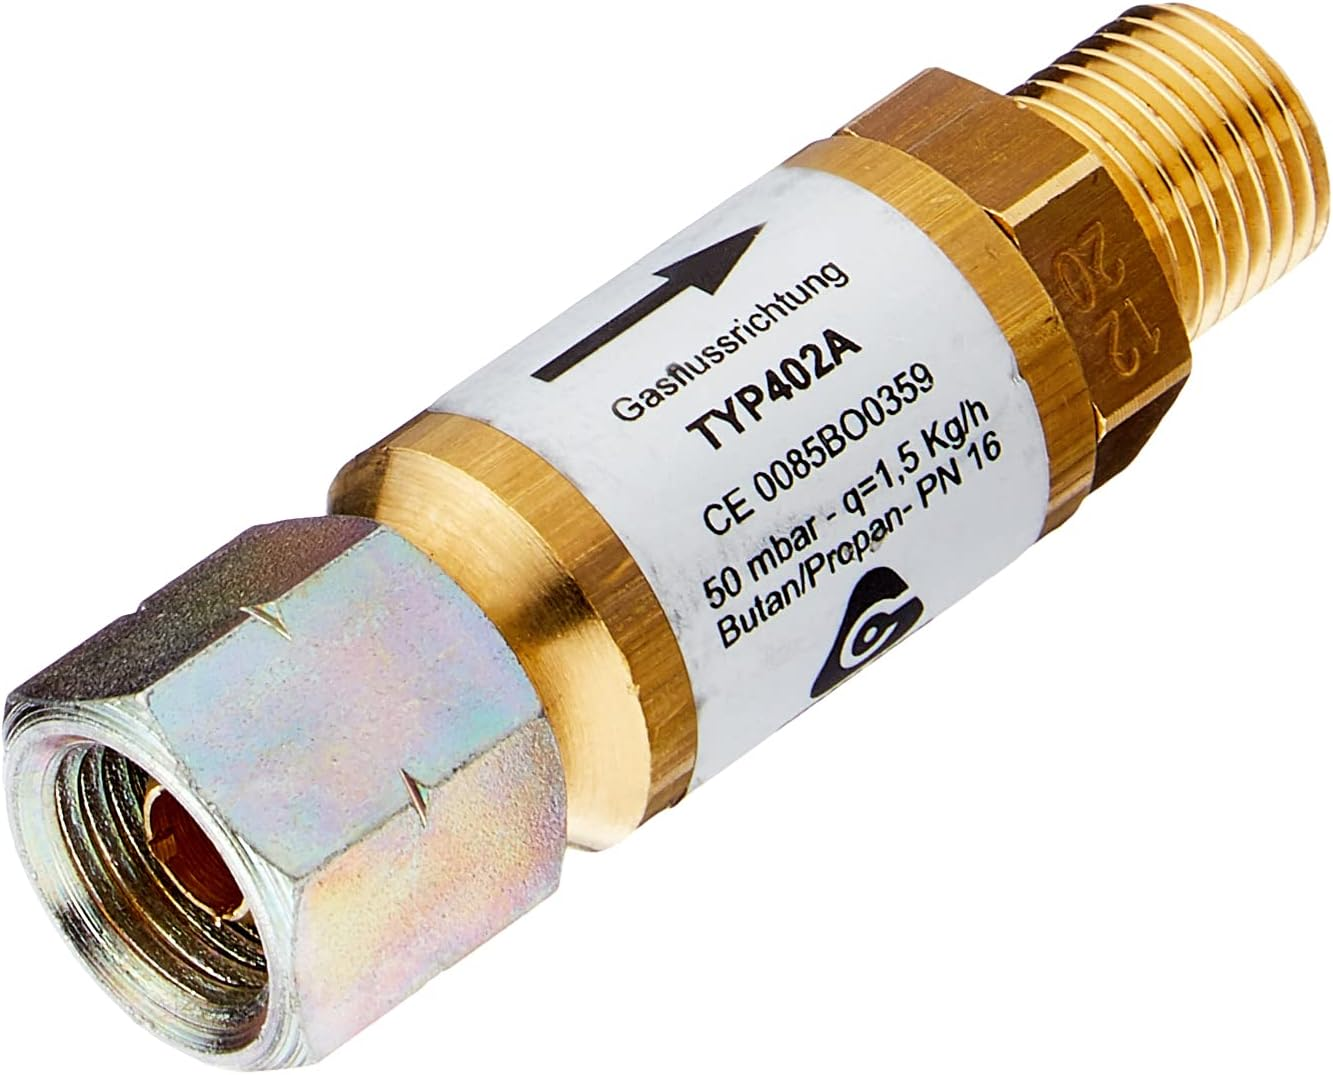
\includegraphics[width=.5\linewidth]{pics/Schlauchbruchsicherung}
		\captionof{figure}{Schlauchbruchsicherung}
		\label{fig:Sicherung}
	\end{minipage}%
	\begin{minipage}{.5\textwidth}
		\centering
		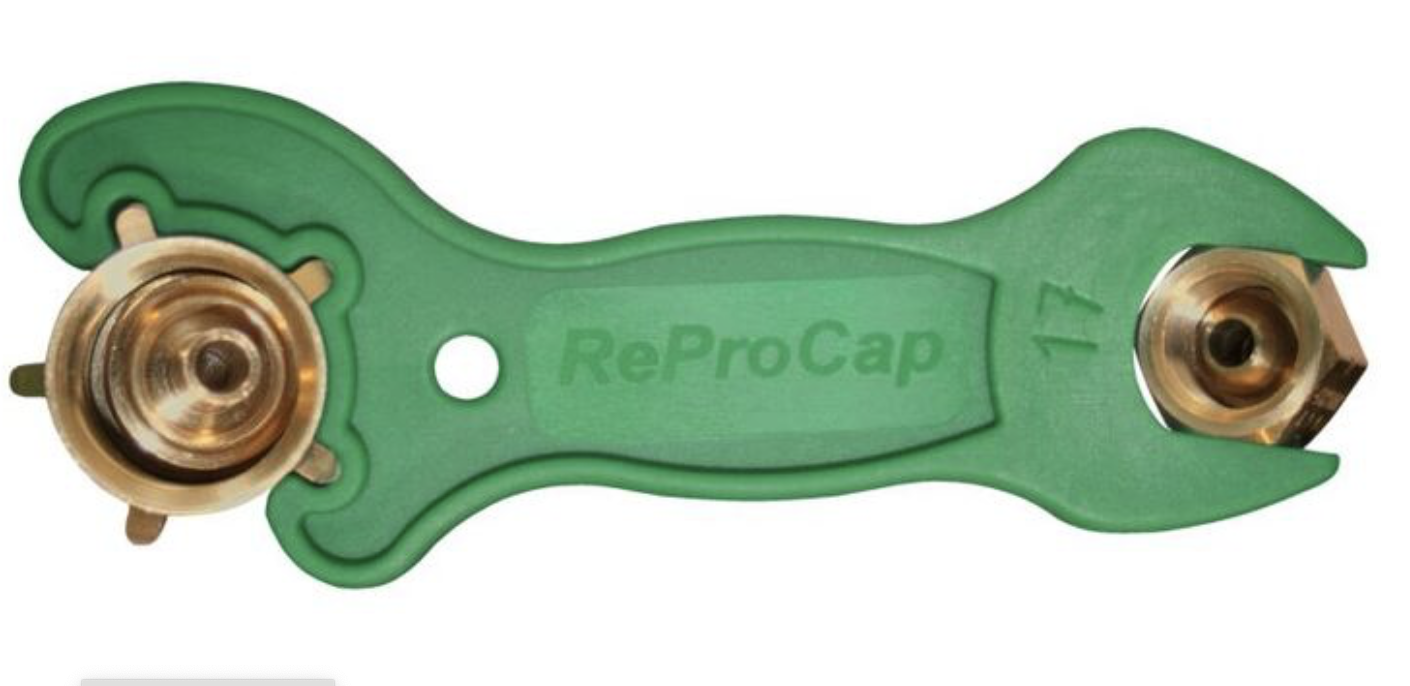
\includegraphics[width=.5\linewidth]{pics/Schlüssel}
		\captionof{figure}{Schlüssel}
		\label{fig:Schlüssel}
	\end{minipage}%
\end{figure}

\subsection{Woran erkenne ich eine gute Qualität?}

	Ich achte immer auf ein paar wenige Merkmale, diese müssen zu meiner 
	Zufriedenheit erfüllt sein, damit ich mich näher mit den Grill beschäftige. 

	\begin{itemize}[noitemsep]
		\item Der Grillrost sollte aus mindestens 6mm starken Edelstahl oder 
	    5mm Gusseisen bestehen. Bei Grillrosts mit 
		geringeren Stärken
		ist es nicht ausgeschlossen, dass sie sich aufgrund der Hitze verformen.
		\item Die Drehgriffe müssen stabil in der Hand liegen, leichtgängig sein und 
		dürfen nicht wackeln. Nichts ist ärgerlicher, als ein Drehgriff, der 
		in seiner Funktion eingeschränkt ist.
		Zum Einem weil die Befestigung unzureichend ist und Griff immer abfällt. 
		Zum Anderen wenn die Kardanwelle nicht mitgenommen wird, weil 
		der Lock beschädigt ist.
		\item Der Deckel sollte schwer ausgeführt und die Scharniere leichtgängig 
		und gut ausbalanciert sein. Bei höherwertigen Grills ist der 
		Deckel doppelwandig, hier sollten auch die
		Seitenteile doppelwandig sein. In der Preisklasse des Napoleon Rogue SE 
		oder XT ist dieses Feature nicht vorgesehen. Der Deckel kann 
		allerdings für kleines Geld gepimt werden. Außerdem sind Reflektoren, die 
		unter den Brennern angebracht werden können eine sinnvolle Ergänzung 
		um die Hitze dort zu halten, wo sie gebraucht wird, in der Grillkammer.
		\item Eine 11kg Gasflasche sollte verwendet werden können. Darf nur die 
		5kg-Gasflasche verwendet werden, obwohl genug Platz für eine 
		11kg-Flasche vorhanden ist,
		ist die Abschirmung nicht stark genug. Auch das ist ein Sicherheits- und 
		Qualitätsmerkmal.
	\end{itemize}

	Eine Kaufberatung und Informationen über die Qualität von Gasgrills bekommt 
	Ihr auf dieser 
	\url{https://www.youtube.com/watch?v=4cMuaoBGZGM }\ {Webseite}

\subsection{Sicheres Handling des Gasgrills} 

	ist nicht selbstverständlich. 
	Hier ein paar Tipps wie man sich auf die 
	sichere Seite stellt. 
	Gasverpuffungen sind nicht so schnuckelig wie sich das Wort Verpuffung 
	anhört. Ganz in Gegenteil, die sind äußerst 
	gefährlich. Deshalb habe ich 
	den Abschnitt auch aufgenommen. Wenn ich euch nix Neues sage ist alles gut, 
	falls es doch etwas Neues für euch gibt ist dieser Absatz notwendig. 

	\begin{itemize}[noitemsep]
	\item Vor dem Anschließen der Gasflasche bitte die Bedienungsanleitung zu 
	Hand nehmen und nachschauen welche 
	Flaschengrößen benutzt 
	werden dürfen. Nicht in jeden Gasgrill darf eine 11kg-Flasche eingebaut 
	werden, obwohl der Platz ausreicht. Es sei 
	euch ans Herz gelegt dieser Vorgabe zu folgen. Denn kein Hersteller der 
	Welt würde schreiben "> Eine 11kg-Flasche darf 
	nicht 
	angeschlossen werden, da das von Ihnen erstandene Gerät zu dünnwandig 
	ist um die Kräfte aufzunehmen, die entstehen 
	wenn 
	das Ventil der Gasflasche durchstartet."<, verständlich, oder? Genau das kann
	der Fall sein und das will niemand.
	\item Ihr habt nun die richtige Gasflasche und wollt diese anschließen. 
	Dabei ist zu bedenken, dass an Gasflaschen aus 
	Sicherheitsgründen ein 
	Linksgewinde verbaut ist. Nachdem auch diese Hürde genommen wurde, 
	stellt sich die Frage, wie bekomme ich das 
	komische Runde Teil, 
	das wie eine Dose aussieht, fest genug an die Flasche geschraubt?  Dafür 
	gibt es spezielle Gasflaschenschlüssel siehe 	
	Abbildung~\vref{fig:Schlüssel}. Um die Dichtigkeit zu überprüfen füllt Ihr 
	eine Wasser-Geschirrspielmittel-Lösung in 
	eine Sprühflasche. 
	Damit besprüht Ihr alle Anschlüsse, wenn Blasen zu sehen sind, ist der 
	Anschluss undicht und muss nachgezogen werden.
	
	\item Wenn alle Anschlüsse dicht sind kann mit dem Grillen begonnen 
	werden. Als erstes müssen die Brenner 
	eingeschaltet werden. Dazu 
	wird der Deckel des Grills geöffnet. Der Drehknopf auf Stellung >>Max.<< 
	gedreht und in Richtung Grill gedrückt, dabei 
	muss ein typisches Knistern und danach das Auflodern der Gasflamme 
	zuhören sein. Bei manchen Modellen ist eine 
	Einschaltsicherung 
	vorhanden, d.h. der Drehknopf muss noch ein paar Sekunden (ca. 5) in der 
	gedrückten Stellung gehalten werden. 
	Ansonsten wird der Gasfluss unterbrochen. Der Grill wird aufgeheizt, sobald 
	der Grill ca. 250 °C hat ist der Rost heiß 
	genug um ihn mit einer 
	Messingbürste abzubürsten.
	\item Ihr habt nun erfolgreich gegrillt und alle sind versorgt, das letzte 
	Grillgut wurde vom Grill genommen. Nun kommt 
	das abschalten. Ich 
	empfehle die Drehregler auf die Position Off zu drehen. Danach die 
	Gasflasche zuzudrehen und dann nochmals einen 
	Brenner zu entzünden,
	sobald das im System vorhandene Gas verbraucht ist geht der Brenner aus 
	und das Gassystem ist drucklos. 
	Der Drehregler des eben benutzten Brenners wieder auf Off stellen. Es 
	strömt kein Gas aus so bald der Drehregler der 
	Gasflasche geöffnet wird, alles gut. 
	Es geht auch so, dass die Gasbrenner noch brennen und die Gasflasche 
	zugedreht wird. Danach auf keinen Fall vergessen 
	die Brenner abzuschalten, da sonst beim nächsten 
	starten des Grills Gas an den Brennern ausströmt kann und es zu der oben 
	erwähnten Verpuffung kommen kann.
\end{itemize}

\begin{figure}[htbp]
	\centering
	\begin{minipage}{1\textwidth}
		\centering
		\includegraphics[width=.9\linewidth]{pics/Gasgrill_Napoleon1}
		\captionof{figure}{Napoleon XT 425}
		\label{fig:Napoleon}
	\end{minipage}
\end{figure}	
\newpage

\section{Der Oberflächengrill}
	
	Ich werde euch den Oberflächengrill von Beefbox (siehe Abbildung~\vref{fig:Beefbox}) vorstellen, da ich dieses 
	Gerät selbst besitze. Der Oberfächengrill ist mit 
	einen 
	Keramikbrenner ausgerüstet, der Oben in der Beefbox sitzt. In der Regel sind 
	die Benner bei den Standalone-Geräten oben 
	angebracht, so dass kein Fett auf den Brenner tropfen kann. Je nach Grillgut 
	kann der Abstand mittels des Einschubs 
	verändert werden. Ich 
	verwende die Beefbox hauptsächlich für Steaks  und Burgerpatties. Durch die 
	hohe Temperatur von ca. 800°C wird das 
	Fleisch von oben angegrillt. Vereinfacht ausgedrückt werden durch die 
	Maillard-Reaktion Röststoffe gebildet. Die Reaktion 
	wurde von Louis Camille 
	Maillard entdeckt. Sie bildet unter dem Einfluss von Hitze mit Eiweißen, 
	reduzierenden Zuckern und der Abspaltung 
	von Wasser die von uns geschätzte Textur und Aromenviefalt. 
	
	Bei dem Oberflächengrill gibt es eine Besonderheit die unbedingt zu beachten 
	ist. Entweder der Grill wird mit einem langen 
	Feuerzeug oder einem
	langen Streichholz entzündet oder mit einer elektrischen Zündung. Es dauert 
	einige Sekunden bis die elektrische Zündung, 
	das Gas entzündet. Dadurch kann es 
	passieren, dass sich Gas in der Garkammer sammelt und bei Entzündung eine 
	Flamme aus der Garkammer schlägt. Die 
	Gefahr dabei ist, dass während des 
	Zündvorgangs in die Garkammer geschaut wird. Das kann schon mal 
	Augenbrauen kosten, oder richtige Verletzungen 
	verursachen. Daher bitte Vorsicht walten 
	lassen. Ansonsten gelten die selben Regeln wie beim Gasgrill.
	
	
	\begin{figure}[htbp]
		\centering
		\begin{minipage}{1\textwidth}
			\centering
			\includegraphics[width=1\linewidth]{pics/Beefbox_Zugeschnitten}
			\captionof{figure}{Beefbox}
			\label{fig:Beefbox}
		\end{minipage}
	\end{figure}	
\newpage

\section{Der Weber Smokey Mountain Water-Smoker}

	Wie auch der Holzkohle-Grill gibt es die Water Smoker in verschiedenen 
	Größen und Ausführungen. Je nach Preissegment in 
	einer mehr oder weniger guten 
	Qualität.
	Außerdem gibt es noch Offset-Smoker, mit Holz oder Pelletbefeuerung, 
	Räucherschränke zum Heiß- und Kalträuchern. 
	Gasgrills mit Räucherschalen, mir ist
	ein Gasgrill bekannt der ein optionales Rauchsystem hat, mit dem die ganze 
	Garkammer gleichmäßig mit Rauch beaufschlagt 
	wird, weitere Informationen über 
	dieses System findet Ihr unter diesen Link 
	\url{https://allgrill.de/allgrill-allrounder-modular/}.
	Ich habe mich für den Smokey Mountain von Weber entschieden, da ich bereits 
	einen Kugelgrill von Weber habe und mit der 
	Qualität des Gerätes sehr zufrieden 
	bin.
	
	Bei dem Smokey Mountain habe ich allerdings zwei Kritikpunkte, die ich nicht 
	verheimlichen will. Der Erste Punkt ist die große 
	Klappe an der Front des Smokers. 
	Die ist aus Aluminium-Blech und macht keinen wertigen Eindruck, außerdem 
	schließt sie nicht wirklich dicht, daher ist mit 
	einem Energieverlust zu rechnen, der 
	durch einen höheren Verbrauch von Brennstoff ausgeglichen werden muss. 
	Außerdem hat der Deckel weder ein Scharnier 
	noch ist eine Möglichkeit, wie beim 
	Kugelgrill, vorhanden um den Deckel
	einzuhängen. Somit muss der Deckel auf den Boden oder eine Ablage gelegt 
	werden. Da dieser Vorgang Zeit kostet geht 
	ebenfalls Hitze verloren, die wieder 
	ausgeglichen werden muss.
	Es gibt Anbieter für Edelstahl-Frontklappen und Scharniere, leider ist das aber 
	mit einer Investition verbunden, die gut und 
	gerne 20\% des Kaufpreises für den 
	Smoker ausmacht.
	
	Der Smokey Mountain Water Smoker von Weber besteht aus einem Kessel, 
	Zwischenstück und einem Deckel. Im Inneren ist 
	ein Kohlerost mit Holzkohle, 
	Wasserschale und zwei übereinander liegende Grillroste für das Gargut zu 
	finden.

\subsection{Anfeuern des Water Smokers}

	Um den Smoker zu befeuern wird der Kohlerost und die Kohlekammer in den 
	Kessel eingesetzt. Der Heizkamin wird zur 
	Hälfte mit Holzkohle befüllt und über 
	einen brennenden Grillanzünder gestellt. Dann wird die Kohlekammer rund um 
	den Kamin mit Holzkohle aufgefüllt. Sobald die 
	Kohle im Kamin durchgeglüht ist 
	wird sie in die Mitte der Kohlekammer geschüttet. Es ist darauf zu achten, dass 
	Kontakt zwischen der Holzkohle in der 
	Kohlekammer mit der durchgeglühten 
	Holzkohle besteht. Das Zwischenstück wird auf den Kessel gestellt und die 
	Wasserschale eingesetzt. Die Wasserschale wird 
	mit vorgeheiztem Wasser befüllt 
	und der Deckel wird geschlossen, die Lüftungsschlitze werden ganz geöffnet 
	damit eine optimale Sauerstoffzufuhr 
	gewährleistet ist. Vor dem Erreichen der 
	Wunschtemperatur sollte der Smoker abgefangen werden, in dem die 
	Lüftungsschlitze fast komplett geschlossen werden. 
	Sobald sich die Temperatur 
	eingependelt hat kann über die Lüftungsschlitze die Feineinstellung erfolgen. 
	
		\begin{figure}[htbp]
		\centering
		\begin{minipage}{1\textwidth}
			\centering
			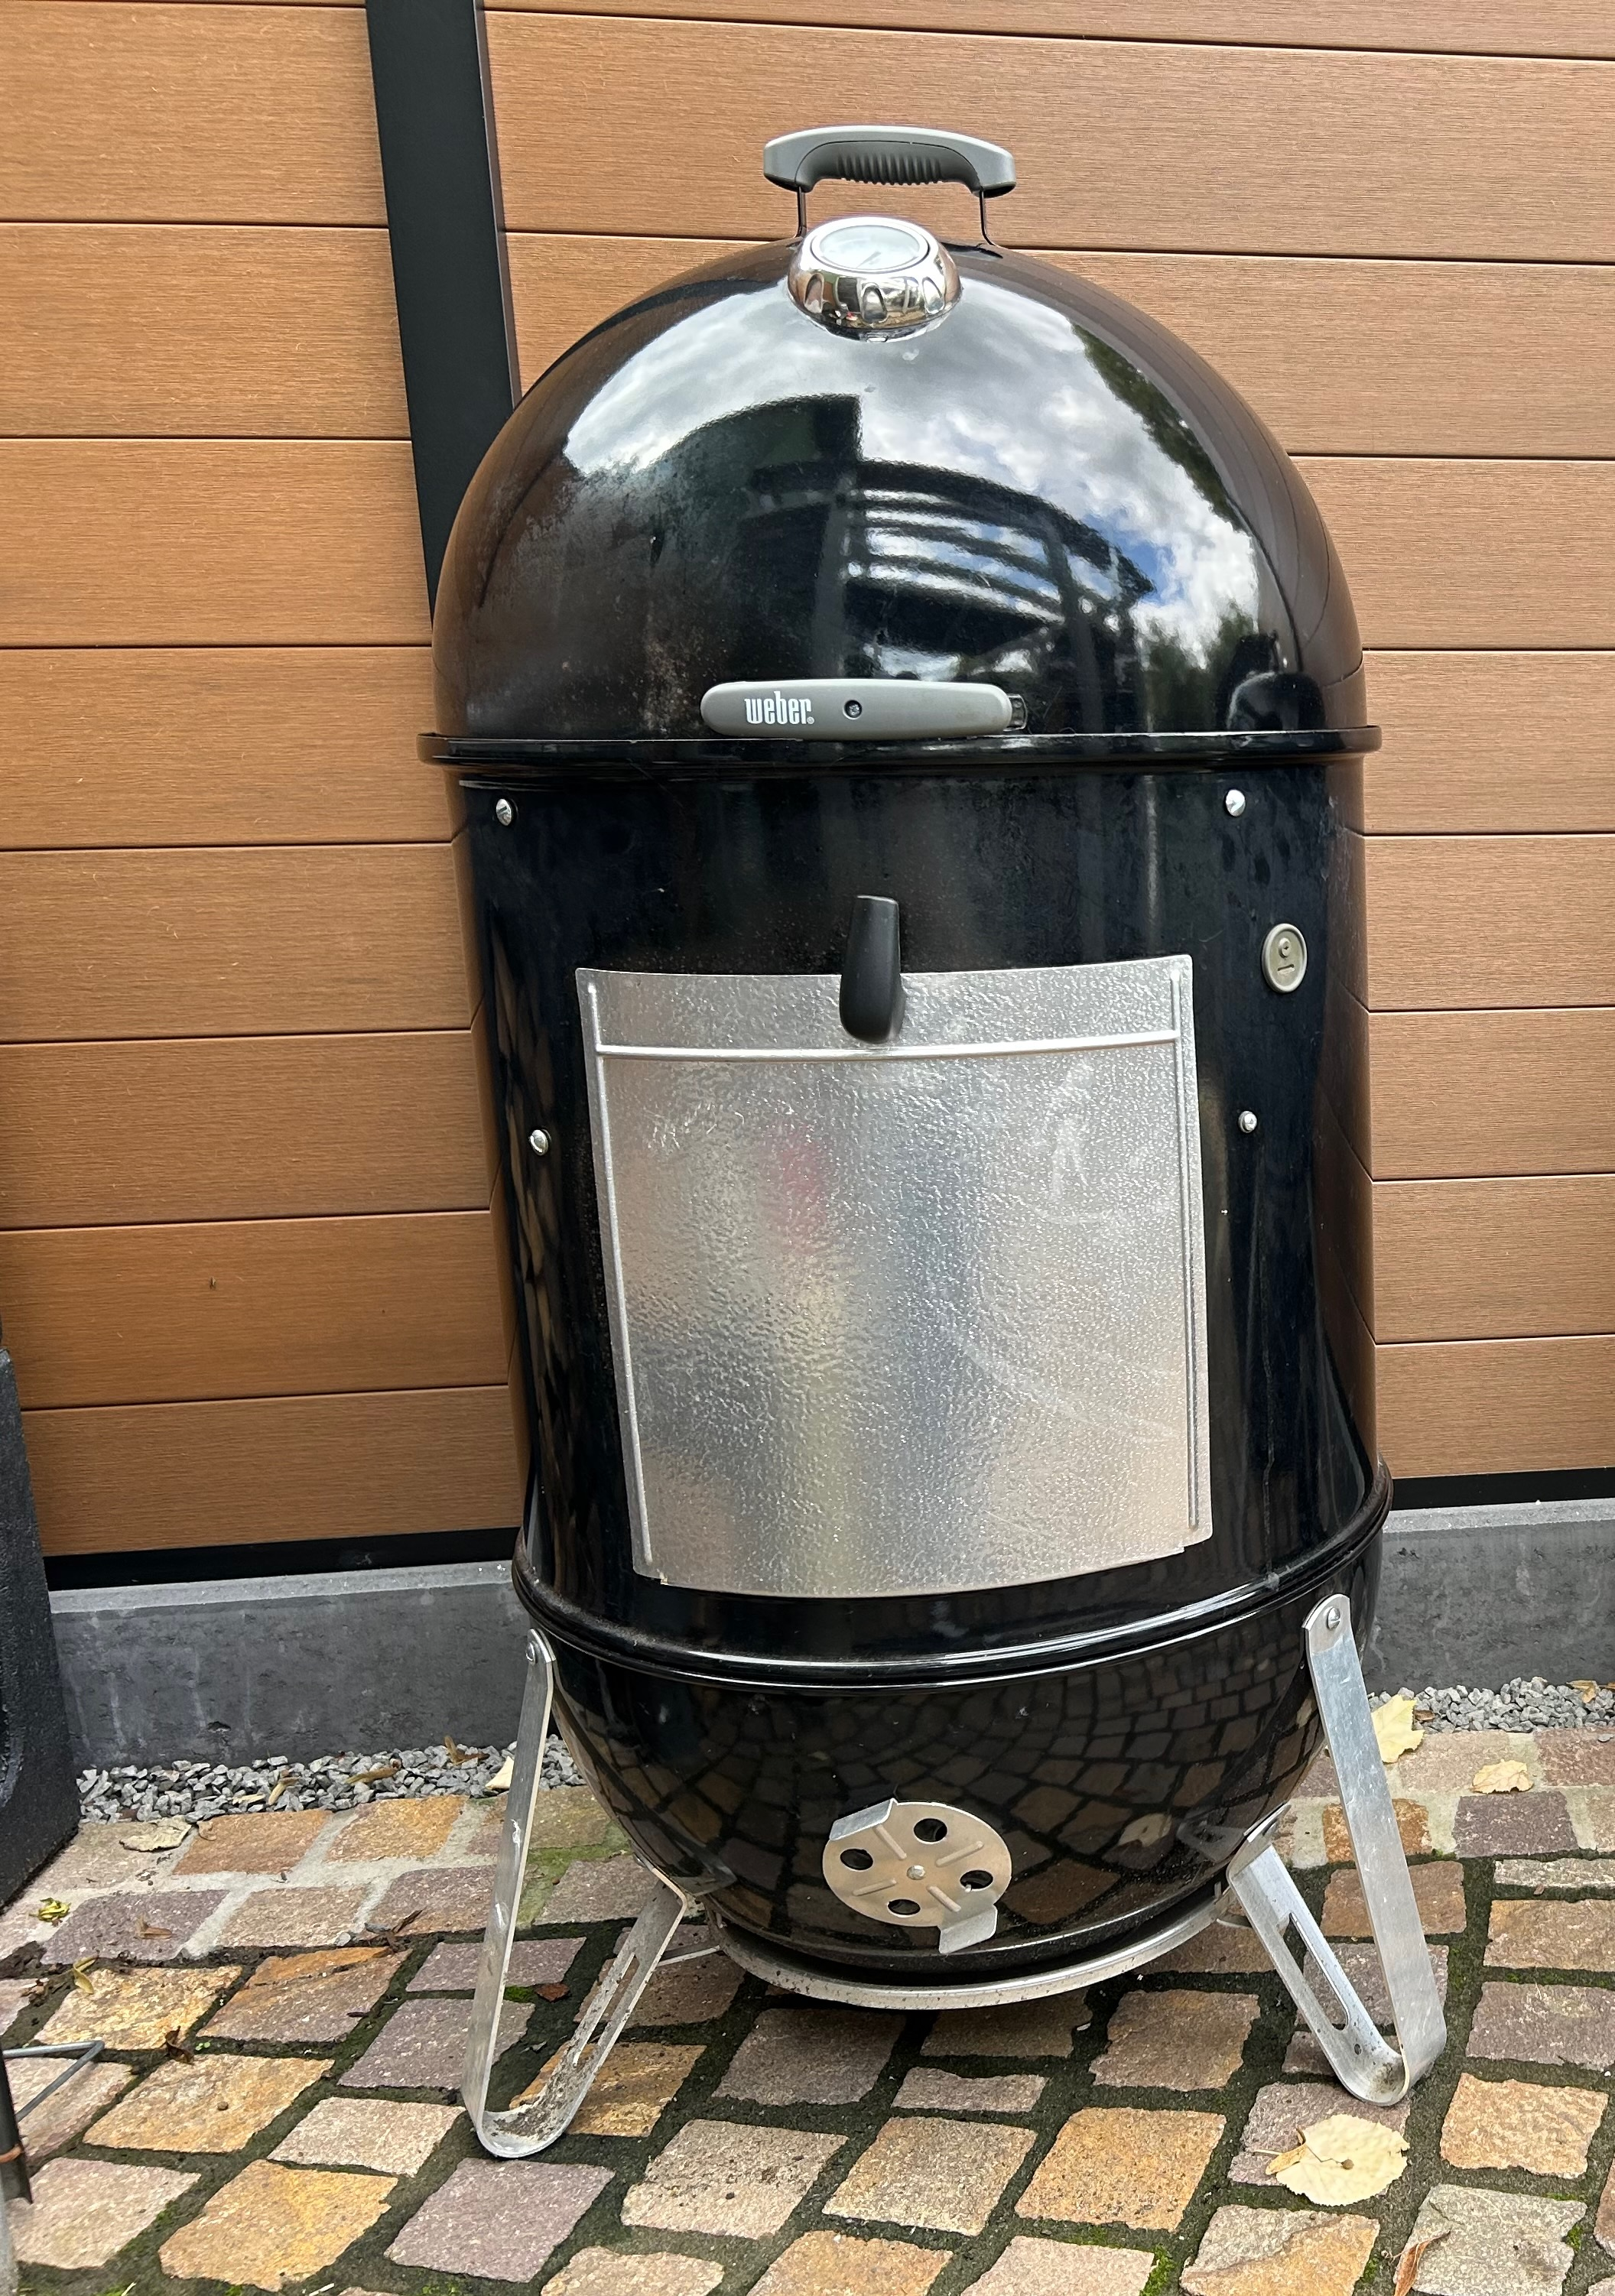
\includegraphics[width=.8\linewidth]{pics/Smoker}
			\captionof{figure}{Weber Water Smoker}
			\label{fig:Smoker}
		\end{minipage}%
	\end{figure}
	\newpage
	